\documentclass[letterpaper]{article}
\usepackage{iccc}
\usepackage{times}
\usepackage{helvet}
\usepackage{courier}
\usepackage{newfloat}
\DeclareFloatingEnvironment[fileext=frm,name=Listing]{listing}
\usepackage[framemethod=tikz]{mdframed}
\mdfsetup{
skipabove=\baselineskip,
skipbelow=0\baselineskip,
innertopmargin=3pt,
innerbottommargin=3pt
}
\usepackage{amssymb,amsmath,amsthm}
\newtheorem{definition}{Definition}
\newtheorem{theorem}{Theorem}
\newtheorem{remark}{Remark}
\usepackage{hetcasl}
%  \usepackage{diagrams}
\usepackage{tikz-cd}
% \usepackage[dvipsnames]{xcolor}
\usepackage{adjustbox}
\usepackage{graphicx}
\usepackage[firstpage]{draftwatermark}
\SetWatermarkText{\shortstack{Draft\\\today\currenttime}}
\SetWatermarkScale{0.75}
\usepackage[T1]{fontenc}
\usepackage{csquotes}
\usepackage[utf8]{inputenc}
\usepackage[british]{babel}
\usepackage[style=apa,natbib,backend=biber,doi=false,url=false]{biblatex}
% \usepackage[style=apa,natbib,backend=biber]{biblatex}
\let\cite\citep
\usepackage[ddmmyyyy]{datetime}
\renewcommand*{\multicitedelim}{\addsemicolon\space}%
\usepackage{xcolor}
\usepackage[
  citebordercolor=white
]{hyperref}

\DeclareLanguageMapping{british}{british-apa}
\addbibresource{papers.bib}
\addbibresource{Corneli_evaluation_bibliography.bib}
\addbibresource{Bou_CoInvent_bibliography.bib}
% \addbibresource{mathsICCC.bib} %
% \addbibresource{danny_bibliothek.bib} %
%% \urlstyle{tt}
\AtBeginBibliography{\def\UrlFont{\footnotesize\tt}}
\renewcommand*{\finalnamedelim}{%
  \ifnumgreater{\value{liststop}}{2}{\finalandcomma}{}%
  \addspace\&\&\space}
\AtEveryCitekey{\renewcommand*{\finalnamedelim}{%
  \ifthenelse{\value{listcount}>\maxprtauth}
    {}
    {\ifthenelse{\value{liststop}>2}
       {\finalandcomma\addspace\bibstring{and}\space}
       {\addspace\bibstring{and}\space}}}}

\AtBeginDocument{\renewcommand\finalandcomma{\addcomma}}
\AtBeginBibliography{%
  \renewcommand*{\finalnamedelim}{%
    \ifthenelse{\value{listcount}>\maxprtauth}
      {}
      {\finalandcomma\addspace\bibstring{and}\space}}}

\newbibmacro{string+doiurlisbn}[1]{%
  \iffieldundef{doi}{%
    \iffieldundef{url}{%
      \iffieldundef{isbn}{%
        \iffieldundef{issn}{%
          #1%
        }{%
          \href{http://books.google.com/books?vid=ISSN\thefield{issn}}{#1}%
        }%
      }{%
        \href{http://books.google.com/books?vid=ISBN\thefield{isbn}}{#1}%
      }%
    }{%
      \href{\thefield{url}}{#1}%
    }%
  }{%
    \href{http://dx.doi.org/\thefield{doi}}{#1}%
  }%
}

\DeclareFieldFormat{title}{\usebibmacro{string+doiurlisbn}{\mkbibemph{#1}}}
\DeclareFieldFormat[inproceedings,article,incollection]{title}%
    {\usebibmacro{string+doiurlisbn}{\mkbibquote{#1}}}

\newcommand{\note}[1]{\begin{quote} \textbf{Note:}  \textit{#1} \end{quote}}
\newcommand{\comment}[1]{\textbf{Comment:}\textit{#1}}
\newcommand{\dannydiv}{\lfloor}

% \pdfinfo{
% /Title (Test)
% /Subject (Proceedings of ICCC)
% /Author (ICCC)}
% The file iccc.sty is the style file for ICCC proceedings.

\title{The role of blending in mathematical invention}

\author{F.\ Bou \\ \Large{\textbf{M.\ Schorlemmer}}\\IIIA - CSIC \\ Barcelona
        \And J. Corneli \\Computing \\Goldsmiths, London
        \And D.\ G{\'o}mez-Ram{\'{\i}}rez\\Cognitive Science \\Osnabr{\"u}ck
        \And E. Maclean \\\Large{\textbf{A.\ Smaill}}\\ Informatics\\ Edinburgh
        \And A. Pease \\ Computing \\ Dundee}


\setcounter{secnumdepth}{0}

\begin{document} 
\maketitle
\begin{abstract}
\begin{quote}
  We model the mathematical process whereby new mathematical theories
  are invented.  Here we
  explain the use of conceptual blending for this purpose, and show
  examples to illustrate the process in action.  Our longer-term goal
  is to support machine and human mathematical creativity.
\end{quote}
\end{abstract}

\section{Introduction}
\label{sec:intro}

We are concerned with creativity in mathematics: creativity
as evinced by human and artificial mathematicians,
individually and collectively.

Work on \emph{conceptual blending} has been much influenced
%by \textcite{Fau98}.
by \textcite{Fau98,FaTu02}.
More recently, the centrality of conceptual blending to creativity
has been stressed by \textcite{MTurner14}, where he writes:
\begin{quote}
  \dots the human spark comes from our advanced ability to \emph{blend} ideas
  to make \emph{new} ideas. Blending is the origin of ideas.%
  \hfill \parencite[p 2]{MTurner14}
\end{quote}
The claim is that blending in this sense is a general human cognitive
ability, and as such applies to mathematics, as much as to art, poetry,
music and so on (see for example \textcite{MTurner05}).

The place of mathematics and the sciences among creative endeavours
has been stressed by the literary critic George Steiner:
\begin{quote}
  It is in mathematics and the sciences that the concepts of
creation and of invention, of intuition and of discovery,
exhibit the most immediate, visible force.
\flushright{\citet[p~145]{Ste01}}
\end{quote}
% A recent survey of examples of blending in mathematics by
% \textcite{Al11i}.  
Blending involves recognising features common
to mathematical concepts, even when expressed in different
terminology.  The role of mathematical analogy in creative mathematics
is well expressed by \textcite{Weil60}, and a general plea for
analogical reasoning within science in \cite{ArbibHesse86}.

We are investigating \emph{computational} accounts of mathematical
creativity, taking conceptual blending as a key ingredient.  The work
%of Goguen \parencite{Gog99,Gog05b,Gog05} 
of \textcite{Gog99,Gog05b} 
has provided a general framework for
comparison of conceptual spaces, and computation of blends.  This
enables the use of richer representation formalisms, and so is closer to
contemporary mathematics than previous computational realisations of
blending, such as in \textcite{Pereira2007}.

This paper deals with the creative process in mathematics, as modelled
along the lines above. We focus on the use of blending within a single
process, searching for blends satisfying some evaluation criteria,
from the starting point of some given conceptual spaces.
% next omitted from camera ready version --
% reviewers request more on the cognitive side, need the space!
% --
% The issues
% involved in social interaction between the agents concerned in more
% realistic scenarios are for consideration elsewhere, but are briefly
% addressed below.

While cognitive issues are important to us, this paper
is focused on issues in representation and representation change;
there are however brief comments on cognition in the conclusions.

We start by providing some background, followed by an example to
illustrate the components involved in our approach. A historical
example based on Georg Cantor's work follows.  The most extended example was
carried out by a pure mathematician (D.\ G{\'o}mez-Ram{\'{\i}}rez), working in a
domain close to his own; in this case, the blend mechanism threw up
some unexpected properties, which provoked new work by the
mathematician.

Subsequently we give some more speculative thoughts on where this work
can go in the future, by considering Galois theory as a test-bed.
Finally, we discuss the evaluation of work along these lines, and
give some conclusions.

%%% Local Variables: 
%%% mode: latex
%%% TeX-master: "mathsICCC"
%%% End: 

\section{Background}
\label{sec:background}

\subsection{Blending in Mathematics}
\label{subsec:mathblend}

%Lakoff and N{\'u}{\~n}ez \citep{Lak00} 
\textcite{Lak00} 
are among the first to present
a cognitive account of the origin and development of mathematical
ideas,\footnote{This is lamented by Lakoff and N{\'u}{\~n}ez, who
claim that (prior to their work), ``there was still no discipline of
mathematical idea analysis from a cognitive perspective''
\citep{Lak00}.} arguing against the ``romance of mathematics'' in which
mathematics is presented as an ever-increasing set of universal,
absolute, certain truths which exist independently of humans. They
present the thesis that human mathematics is grounded in bodily
experience of a physical world, and mathematical entities inherit
properties which objects in the world have, such as being consistent
or stable over time.  Exploring the physical world of object
collection might lead to concepts like the empty collection and rules
like ``adding a collection of $n$ objects to an empty collection
yields a collection with $n$ objects''. People then form grounding
metaphors between the physical world and an abstract mathematical
world, allowing us to project from everyday experiences onto abstract
concepts, thus leading to the concept of zero and the axiom that $n +
0 = n$. Lakoff and N{\'u}{\~n}ez posit that blending different
mathematical metaphors leads to more complex ideas (see
also~\textcite{alexander11}). 

Alongside this account of mathematical cognition, mainstream
contemporary mathematics has developed its own methodology and
foundations, enjoying an exceptional place among scientific
disciplines. Its methods, objects of study and sometimes astonishing
results have widespread, if not universal, acceptance.

In conclusion, mathematics is a scientific discipline having not only
a fundamental cognitive component, necessary in its development, but
also possessing a collection of general principles and structures
going beyond a particular school of thought.  Among these general
processes we want to highlight in this paper the importance that
conceptual blending has in mathematics, incorporating both cognitive and
mathematically specific aspects in order to create new mathematical concepts.


%% \subsection{Some mathematical concepts}
%% In this paper we draw on Lakoff and N{\'u}{\~n}ez's ideas to produce a
%% computational model of blending in abstract mathematics. We present
%% three illustrative examples: the mathematical notion of infinity,
%% prime ideals and Galois theory. The first of these is the idea of a
%% number, process etc without limits or end. The latter two are concepts
%% from abstract algebra, which explores groups and related objects and
%% their properties. 

%% A {\em prime ideal} is a subset of a ring, which certain
%% properties, and Galois theory draws an important connection between
%% fields and groups, which can be used to simplify problems in field
%% theory. 

\subsection{Terminology for conceptual blending}
Our notion of conceptual blending is informed by Category theory, and
highly influenced by Goguen's work on concepts \parencite{Gog05b}. In
this paper we use the terminology below, and elucidate the terminology
by means of a running example -- discovering a version of the integers
(in the sense of providing a partial approach to the genuine integers)
using blending.

{\bf Conceptual spaces} are partial and temporary representational
structures which are constructed on the fly when talking about a
particular situation, which are informed by the knowledge structures
associated with a domain. These are influenced by Boden's idea of a
concept space which is mapped, explored and transformed by
transcending mapped boundaries \parencite{boden}, and form the input spaces
to our blend. 

As an example of two conceptual spaces, consider one as a theory
$\SIdIndex{NAT}$ --
a theory of the natural numbers, and $\SIdIndex{FUNC}$ -- a theory of a total
unary function with an inverse. 
%The terminology here used obviously refers to the fact that these two
%conceptual spaces are partial representations of the genuine concepts
%employed by mathematicians.  
We will refer back to these theories in this exposition.

(Many-sorted) First-order {\bf Axioms} are the criteria which will be
used here to delineate the conceptual
spaces. The axiomatic method has been a fundamental aspect of
mathematical research since Euclid, and various axiom changes have led
to revolutions in mathematics. For instance, 
%relaxing the axioms
%defining numbers led to negative and imaginary numbers, and 
rejecting
the parallel postulate opened up fascinating new areas of
non-Euclidean geometry.

The precise formulations for $\SIdIndex{NAT}$ and $ \SIdIndex{FUNC}$ can
be found in Listings~\ref{fig:nats} and \ref{fig:inv}. 
Notice that these formulations obviously refer to 
%the fact that these two conceptual spaces are 
partial representations of the genuine concepts
employed by mathematicians.  
In the conceptual space with theory $\SIdIndex{NAT}$, an example of an axiom is 
%$\forall x. \neg s(x) = 0$ -- that is that zero is not a successor element.
$\forall x. \neg \: 0 = \Id{s}(x)$ -- that is that zero is not a successor element.
%the least element of the natural numbers. 
The conceptual space with theory $\SIdIndex{FUNC}$ has an axiom
%$\forall x.\;f(f^{-1}) x = x$. 
$\forall x.\:\:\Id{f}(\Id{finv}(x)) = x$. 
%where heuristics for transformation, such as {\em consider
%the negative} and {\em drop a constraint}, are suggested.

{\bf Signature morphisms} between conceptual spaces are mappings from
the symbols of the source conceptual space into the symbols of the other
conceptual space. 
%
%For example $\SIdIndex{NAT}$ contains a function $\lambda
%x:\Id{Nat}.\;\Id{s}(x)$ to denote the successor, and $\SIdIndex{FUNC}$ contains a function
%$\lambda x:\Id{X}.\;\Id{f}(x)$. 
%A theory $G$ common to both may contain a function
%%$\lambda x:\sigma.\;g(x)$. 
%$\lambda x:\Id{N}.\;\Id{func}(x)$. 
For example $\SIdIndex{NAT}$ contains a function $\lambda
x:\Id{Nat}.\;\Id{s}(x)$ that maps $x$ to its successor, and
$\SIdIndex{FUNC}$ contains a function defined over a set $X$ that maps
each element to an image $\lambda x:\Id{X}.\;\Id{f}(x)$.  A theory $G$
with a morphism to both $\SIdIndex{NAT}$ and $\SIdIndex{FUNC}$ might
contain a function $\lambda x:\Id{N}.\;\Id{func}(x)$ that takes every
number in some set $\Id{N}$ to its image under $\Id{func}$.
%
When we show a mapping % in this paper 
we write 
this as
\begin{align}
  \Id{s}&&\leftarrow_{\phi(G,\SIdIndex{NAT})}&&\Id{func}&&\rightarrow_{\phi(G,\SIdIndex{FUNC})}&&\Id{f}\\
  \Id{Nat}&&\leftarrow_{\phi(G,\SIdIndex{NAT})}&&\Id{N}&&\rightarrow_{\phi(G,\SIdIndex{FUNC})}&&\Id{X}
\end{align}
\noindent The mapping $\phi(G,\SIdIndex{NAT})$ is a signature morphism from
$G$ to $\SIdIndex{NAT}$. Note that associated types are also mapped.

{\bf Input Spaces} refer to two or more conceptual spaces of
interest. 

{\bf Generic spaces} are conceptual spaces that possess commonality
between input spaces. 

%{\bf Colimits} are conceptual spaces representing a blend of input
%spaces with respect to a given generic space and set of signature
%morphisms. These are uniquely computed given a generic space and set of
%morphisms. Here is a diagrammatic representation of such a computation
%in our example using theories $\SIdIndex{NAT}$ and $\SIdIndex{FUNC}:$
{\bf Colimits} are conceptual spaces representing a blend of input
spaces with respect to a given generic space and a set of signature
morphisms. These are uniquely computed given a generic space and a set of
morphisms. Here is a diagrammatic representation of such a computation
in our example using theories $\SIdIndex{NAT}$ and $\SIdIndex{FUNC}:$
%\begin{center}
%  \begin{diagram}[size=7mm]
%    &       &   $G$   &       & \\
%    & \ldTo^{\rotatebox{-45}{$\phi(G,\SIdIndex{NAT})$}} &       &
%    \rdTo^{\rotatebox{45}{$\phi(G,\SIdIndex{FUNC})$}} &          \\
%    \SIdIndex{$\SIdIndex{NAT}$} &       &   &       &
%    \SIdIndex{$\SIdIndex{FUNC}$} \\
%    & \rdTo_{\rotatebox{45}{$\phi(B,\SIdIndex{NAT})$}} &       &
%    \ldTo_{\rotatebox{-45}{$\phi(B,\SIdIndex{FUNC})$}} &  \\
%    & & $Colimit$ & & 
%  \end{diagram}
%\end{center}
\begin{center}
  \begin{tikzcd}[column sep=normal, row sep=small]
    & \textrm{Colimit}
    \\
    \SIdIndex{NAT} \arrow{ur}{\phi(B,\SIdIndex{NAT})} & & \SIdIndex{FUNC} \arrow{ul}[swap]{\phi(B,\SIdIndex{FUNC})} \\
    & G \arrow{ul}{\phi(G,\SIdIndex{NAT})}
    \arrow{ur}[swap]{\phi(G,\SIdIndex{FUNC})}
  \end{tikzcd}
\end{center}
The conceptual space represented by the Colimit is often referred to
as the {\em blend}. 

{\bf Internal Evaluation} constitutes a variety of techniques to determine whether a computed colimit is viable as a conceptual space. In our example, since the conceptual spaces are mathematical theories, we can exploit the notion of consistency. This is a way of evaluating whether a
blend is not only creative, but also valid. In the example of theories
$\SIdIndex{NAT}$ and $\SIdIndex{FUNC}$,
the computed blend is inconsistent due to the emergent axioms in the
computed colimit. The only type existing within the colimit is from now
on referred to as $\mathbb{Z}$ to distinguish it from the natural
numbers. Notice that in the colimit it holds that:
%\begin{eqnarray*}
%  \forall x: \mathbb{Z}. \neg\; \Id{zero} &=&\Id{s}(x)\\
%%\forall x:\mathbb{Z}.\;s(s^{-1}( x)) &=& x
%\forall x:\mathbb{Z}.\; \Id{s}(\Id{sinv}( x)) &=& x
%\end{eqnarray*}
%\[
%  \begin{array}{lc@{\: = \:}c}
%    \forall x: \mathbb{Z}. \neg & \Id{zero} & \Id{s}(x)\\
%    \forall x: \mathbb{Z}. & \Id{s}(\Id{sinv}(x)) & x \\
%  \end{array}
%\]
\begin{center}
  $\forall x: \mathbb{Z}. \neg \:\:   \Id{zero} = \Id{s}(x)$
\end{center}
\begin{center}
  $\forall x: \mathbb{Z}. \:\: \Id{s}(\Id{sinv}(x)) = x$ \:.
\end{center}
This is an inconsistency, as from the second axiom we see 
that there is an
element for which 0 is the successor.

{\bf Weakening} refers to the process of weakening the input
theories by removing symbols or axioms. If we remove the axiom 
$$
\forall x: \Id{Nat}. \neg \:\: \Id{zero} = \Id{s}(x)
$$
then the resulting computed colimit contains a mathematical theory
which is consistent.  

\textcite{MartinezEtAl14} provides an algorithm to explore the space
of blends resulting from given input spaces and a given generic space, where
weakening is achieved by omitting axioms.  The algorithm returns the
blends which are consistent, and maximally so, among those in this
space of blends.  This algorithm assumes that consistency of relevant
theories can be checked, so is not always effective.

{\bf Running the blend} refers to elaborating or completing a
mathematical theory. Sometimes there are missing definitions which
need to be discovered. For example in the new theory 
%the following axioms exists
the following axiom appears
\begin{eqnarray*}
%\forall x,y:\mathbb{Z}. \: s(x) + y &=& s(x+y)
  \forall x,y:\mathbb{Z}. \:\: \Id{s}(x) + y &=& \Id{s}(x+y) \:,
\end{eqnarray*}
%but we also are interested in additional axioms such as
but we also are interested in theorems such as
\begin{eqnarray*}
%\forall x,y:\mathbb{Z}. s^{-1}(x) + y &=& s^{-1}(x+y)
  \forall x,y:\mathbb{Z}. \:\: \Id{sinv} (x) + y &=& \Id{sinv} (x+y) \:.
\end{eqnarray*}
Finding suitable theorems is an example of running the blend, and from which it
is possible to discover and prove 
%such 
theorems such as
\begin{eqnarray*}
%\forall x,y:\mathbb{Z}. s^{-1}(x) + s(y) &=& x+y
  \forall x,y:\mathbb{Z}. \:\: \Id{sinv}(x) + \Id{s}(y) &=& x+y \:.
\end{eqnarray*}

\subsection{Technologies}

The approach explained above corresponds to Goguen's
proposal \parencite{Gog99} for implementing blending, but slightly
simplified % (as in \textcite{Kutz2012} and \textcite{KuMoNeCo14}): 
(as in \textcite{KuMoNeCo14}): 
we use
the normal colimit construction, rather than $\frac{3}{2}$-colimits
(both described in \textcite{Gog99}).

%In the examples here considered we will be using colimits of V-shaped
%diagrams (cf.~Figure??). Thus, in each of the cases we have to specify
%two morphisms between a source conceptual space and a target conceptual
%space, with the restriction that both morphisms share the same source
%conceptual space.

Additionally we assume that the conceptual spaces involved are % always
given using a CASL specification \parencite{astesiano2002casl} and that the
morphisms are theorem preserving (i.e.\ map theorems to theorems).
% (but perhaps not axiom preserving). 
The reason for these assumptions is that in these cases
it is well-known how to compute % colimits \parencite{Mo98a}; 
colimits: the colimit
specification essentially corresponds to the disjoint union of the two
target conceptual spaces except for not repeating the symbols given in
the common source conceptual space.  Moreover, we will be using the
HETS system \parencite{MossakowskiEA06} to compute such colimits.
The code for the implemented examples in this paper
is available on-line.%
\footnote{See: \texttt{\url{https://github.com/ewenmaclean/ICCC2015_hetsfiles}}}

The use of CASL specifications means that we deal with first-order
logic; CASL is supported in the HETS system, and colimits here can be
computed in the current implementation of HETS. Although higher-order
logic (with Henkin semantics) is available in HETS (indeed in CASL)
and the colimits are well-known to exist (because higher-order in this
form is reducible to many-sorted first-order logic), it is worth
noticing that the calculus of such colimits is not currently available
in HETS.  This restricts the formalisms that can be used directly for
our purposes, where computation of colimits is central to our
approach.


%%% Local Variables: 
%%% mode: latex
%%% TeX-master: "mathsICCC"
%%% End: 

\section{Blending and the infinite}
\label{sec:infinity}

\note{Marco, Ewen, Alan, Felix}


In this paper we want to follow Goguen's proposal \cite{Go99c} for
implementing blending, but slightly simplified (like in
\cite{KuMoHoBhBa12}): we will only deal with
the well-known notion of colimit in a category \cite{Gog91}, instead of
using $\frac{3}{2}$-colimits.

In the examples here considered we will be using colimits of V-shaped
diagrams (cf.~Figure??). Thus, in each of the cases we have to specify
two morphisms between a source conceptual space and a target conceptual
space, with the restriction that both morphisms share the same source
conceptual space.

Additionally we will assume that the involved conceptual spaces are
always given using a
CASL specification \cite{MoHaSaTa08} and that the morphisms are theorem
preserving (but perhaps not axiom preserving). The reason to these
assumptions
is that in these cases it is well-known how to compute colimits
\cite{Mo98a}; the colimit specification essentially corresponds to the
disjoint union of the two target conceptual spaces except for not
repeating the symbols given in the common source conceptual space.
Moreover, we will be using 
the HETS system \parencite{MossakowskiEA06} to compute such colimits.



\subsection{Naturals and Integers}

\subsection{A Simple Example -- the Integers}

As a first demonstration of the machinery involved in blending
mathematical theories, we consider combining a theory of natural
numbers with the concept of the inverse of a function to obtain the
integers. Let us assume an simple axiomatisation of the natural
numbers (without order axioms) as shown in Figure \ref{fig:nats}, and
call this theory $\SIdIndex{Nat}$. Now let us also define a simple theory
which introduces the concept of a function with an inverse as shown in
Figure \ref{fig:inv}, and call this theory $\mathbb{F}$. 
\begin{figure}[!ht]
\begin{hetcasl}
\SPEC \=\SIdIndex{Nat} \Ax{=}\\
\> \SORT \Id{Nat}\\
\> \OPS \=\Id{zero} \Ax{:} \Id{Nat};\\
\>\> \Id{s} \Ax{:} \=\Id{Nat} \Ax{\rightarrow} \Id{Nat};\\
\>\> \Ax{\_\_}\Ax{+}\Ax{\_\_} \Ax{:} \=\Id{Nat} \Ax{\times} \Id{Nat} \Ax{\rightarrow} \Id{Nat}\\
\> \Ax{\forall} \=\Id{x}, \Id{y}, \Id{z} \Ax{:} \Id{Nat} \\
\> \Ax{\bullet} \=\Id{s}(\Id{x}) \Ax{=} \Id{y} \Ax{\wedge} \=\Id{s}(\Id{x}) \Ax{=} \Id{z} \Ax{\Rightarrow} \=\Id{y} \Ax{=} \Id{z}\\
\> \Ax{\bullet} \=\Id{s}(\Id{x}) \Ax{=} \Id{s}(\Id{y}) \Ax{\Rightarrow} \=\Id{x} \Ax{=} \Id{y}\\
\> \Ax{\bullet} \=\Ax{\exists} \Id{a} \Ax{:} \Id{Nat} \Ax{\bullet} \=\Id{s}(\Id{x}) \Ax{=} \Id{a}\\
\> \Ax{\bullet} \Ax{\neg} \=\Id{s}(\Id{x}) \Ax{=} \Id{zero}\\
\> \Ax{\bullet} \=\Id{s}(\Id{x}) \Ax{+} \Id{y} \Ax{=} \Id{s}(\=\Id{x} \Ax{+} \Id{y})\\
\> \Ax{\bullet} \=\Id{zero} \Ax{+} \Id{y} \Ax{=} \Id{y}\\
\KW{end}
\end{hetcasl}
\caption{A theory of the natural numbers without order}
\label{fig:nats}
\end{figure}

\begin{figure}[!ht]
\begin{hetcasl}
\SPEC \=\SIdIndex{Func} \Ax{=}\\
\> \SORT \Id{X}\\
\> \OP \=\Id{f} \Ax{:} \=\Id{X} \Ax{\rightarrow} \Id{X}\\
\> \OP \=\Id{finv} \Ax{:} \=\Id{X} \Ax{\rightarrow} \Id{X}\\
\> \Ax{\forall} \=\Id{x} \Ax{:} \Id{X} \\
\> \Ax{\bullet} \=\Id{f}(\Id{finv}(\Id{x})) \Ax{=} \Id{x}\\
\> \Ax{\bullet} \=\Id{finv}(\Id{f}(\Id{x})) \Ax{=} \Id{x}\\
\KW{end}
\end{hetcasl}
\caption{A theory with a function and its inverse defined}
\label{fig:inv}
\end{figure}



\subsubsection{Identifying a Generic Space}
In order to incorporate the notion of blending here we want to be able
to identify a ``generic'' component of each theory and compute the
colimit (also known as pushout) as discusses in \S\ref{sec:background}. We can use the
HDTP system \parencite{GustKS2006,Schmidt2010} to discover a common theory
and signature morphism between symbols in the
two theories $\SIdIndex{Nat}$ and $\SIdIndex{Fun}$. The Generic theory
contains a sort $N$ and a function $func$, and the morphisms from the
Generic theory to $\SIdIndex{N}$ and $\SIdIndex{Fun}$ are:
\begin{align}
s&&\leftarrow_{g_\SIdIndex{Nat}}&&func&&\rightarrow_{g_\SIdIndex{Fun}}&&f\\
Nat&&\leftarrow_{g_\SIdIndex{Nat}}&&N&&\rightarrow_{g_\SIdIndex{Fun}}&&X
\end{align}
Here the successor function is identified in the mapping with the
function in the theory $\SIdIndex{Fun}$, and $g_K$ is the label for
the set of symbol mappings determined by the signature morphism from
the Generic space the theory $K$.

\subsubsection{Computing the Colimit}
The HETS system \parencite{MossakowskiEA06} can then be exploited to
find a new theory by computing the colimit:
\begin{center}
  \begin{diagram}[size=7mm]
    &       &   $Gen$   &       & \\
    & \ldTo^{\rotatebox{-45}{$g_\SIdIndex{Nat}$}} &       &
    \rdTo^{\rotatebox{45}{$g_\SIdIndex{Fun}$}} &          \\
    \SIdIndex{Nat} &       &   &       & \SIdIndex{Fun} \\
    & \rdTo_{\rotatebox{45}{$b_\SIdIndex{Nat}$}} &       &
    \ldTo_{\rotatebox{-45}{$b_\SIdIndex{Fun}$}} &  \\
    & & $Blend$ & &
  \end{diagram}
\end{center}
This generates the theory shown in \ref{fig:inconsistentintegers}.

\begin{figure}[!ht]
\begin{hetcasl}
\SPEC \=\SIdIndex{Spec} \Ax{=}\\
\> \SORT \Id{N}\\
\> \OP \=\Ax{\_\_}\Ax{+}\Ax{\_\_} \Ax{:} \=\Id{N} \Ax{\times} \Id{N} \Ax{\rightarrow} \Id{N}\\
\> \OP \=\Id{p} \Ax{:} \=\Id{N} \Ax{\rightarrow} \Id{N}\\
\> \OP \=\Id{s} \Ax{:} \=\Id{N} \Ax{\rightarrow} \Id{N}\\
\> \OP \=\Id{zero} \Ax{:} \Id{N}\\
\> \Ax{\forall} \=\Id{x}, \Id{y}, \Id{z} \Ax{:} \Id{N} \=\Ax{\bullet} \=\Id{s}(\Id{x}) \Ax{=} \Id{y} \Ax{\wedge} \=\Id{s}(\Id{x}) \Ax{=} \Id{z} \Ax{\Rightarrow} \=\Id{y} \Ax{=} \Id{z} \`{\small{}\KW{\%}(Ax1)\KW{\%}}\\
\> \Ax{\forall} \=\Id{x}, \Id{y} \Ax{:} \Id{N} \=\Ax{\bullet} \=\Id{s}(\Id{x}) \Ax{=} \Id{s}(\Id{y}) \Ax{\Rightarrow} \=\Id{x} \Ax{=} \Id{y} \`{\small{}\KW{\%}(Ax2)\KW{\%}}\\
\> \Ax{\forall} \=\Id{x} \Ax{:} \Id{N} \=\Ax{\bullet} \=\Ax{\exists} \Id{a} \Ax{:} \Id{N} \Ax{\bullet} \=\Id{s}(\Id{x}) \Ax{=} \Id{a} \`{\small{}\KW{\%}(Ax3)\KW{\%}}\\
\> \Ax{\forall} \=\Id{x} \Ax{:} \Id{N} \=\Ax{\bullet} \Ax{\neg} \=\Id{s}(\Id{x}) \Ax{=} \Id{zero} \`{\small{}\KW{\%}(Ax4)\KW{\%}}\\
\> \Ax{\forall} \=\Id{x}, \Id{y} \Ax{:} \Id{N} \=\Ax{\bullet} \=\Id{s}(\Id{x}) \Ax{+} \Id{y} \Ax{=} \Id{s}(\=\Id{x} \Ax{+} \Id{y}) \`{\small{}\KW{\%}(Ax5)\KW{\%}}\\
\> \Ax{\forall} \=\Id{y} \Ax{:} \Id{N} \=\Ax{\bullet} \=\Id{zero} \Ax{+} \Id{y} \Ax{=} \Id{y} \`{\small{}\KW{\%}(Ax6)\KW{\%}}\\
\> \Ax{\forall} \=\Id{x} \Ax{:} \Id{N} \=\Ax{\bullet} \=\Id{s}(\Id{p}(\Id{x})) \Ax{=} \Id{x} \`{\small{}\KW{\%}(Ax1\Ax{\_}7)\KW{\%}}\\
\> \Ax{\forall} \=\Id{x} \Ax{:} \Id{N} \=\Ax{\bullet}
\=\Id{p}(\Id{s}(\Id{x})) \Ax{=} \Id{x}
\`{\small{}\KW{\%}(Ax2\Ax{\_}8)\KW{\%}}
\end{hetcasl}
\caption{An inconsistent version of the integers (without order)}
\label{fig:inconsistentintegers}
\end{figure}


\subsubsection{Removal of Inconsistencies}
This theory is automatically determined to be inconsistent due to the axioms
\begin{eqnarray}
\forall x : \mathbb{Z} . not s(x) &=& 0 \label{eq:limnat1}\\
s(p(x)) &=& x \label{eq:sucpre}
\end{eqnarray}
Removal of the limiting axiom (\ref{eq:limnat1}) results in a theory which is very
similar to what we understand to be the integers as shown in Figure~\ref{fig:integers}.
\begin{figure}[!ht]
\begin{hetcasl}
\SPEC \=\SIdIndex{Spec} \Ax{=}\\
\> \SORT \Id{N}\\
\> \OP \=\Ax{\_\_}\Ax{+}\Ax{\_\_} \Ax{:} \=\Id{N} \Ax{\times} \Id{N} \Ax{\rightarrow} \Id{N}\\
\> \OP \=\Id{p} \Ax{:} \=\Id{N} \Ax{\rightarrow} \Id{N}\\
\> \OP \=\Id{s} \Ax{:} \=\Id{N} \Ax{\rightarrow} \Id{N}\\
\> \OP \=\Id{zero} \Ax{:} \Id{N}\\
\> \Ax{\forall} \=\Id{x}, \Id{y}, \Id{z} \Ax{:} \Id{N} \=\Ax{\bullet} \=\Id{s}(\Id{x}) \Ax{=} \Id{y} \Ax{\wedge} \=\Id{s}(\Id{x}) \Ax{=} \Id{z} \Ax{\Rightarrow} \=\Id{y} \Ax{=} \Id{z} \`{\small{}\KW{\%}(Ax1)\KW{\%}}\\
\> \Ax{\forall} \=\Id{x}, \Id{y} \Ax{:} \Id{N} \=\Ax{\bullet} \=\Id{s}(\Id{x}) \Ax{=} \Id{s}(\Id{y}) \Ax{\Rightarrow} \=\Id{x} \Ax{=} \Id{y} \`{\small{}\KW{\%}(Ax2)\KW{\%}}\\
\> \Ax{\forall} \=\Id{x} \Ax{:} \Id{N} \=\Ax{\bullet} \=\Ax{\exists} \Id{a} \Ax{:} \Id{N} \Ax{\bullet} \=\Id{s}(\Id{x}) \Ax{=} \Id{a} \`{\small{}\KW{\%}(Ax3)\KW{\%}}\\
\> \Ax{\forall} \=\Id{x}, \Id{y} \Ax{:} \Id{N} \=\Ax{\bullet} \=\Id{s}(\Id{x}) \Ax{+} \Id{y} \Ax{=} \Id{s}(\=\Id{x} \Ax{+} \Id{y}) \`{\small{}\KW{\%}(Ax4)\KW{\%}}\\
\> \Ax{\forall} \=\Id{y} \Ax{:} \Id{N} \=\Ax{\bullet} \=\Id{zero} \Ax{+} \Id{y} \Ax{=} \Id{y} \`{\small{}\KW{\%}(Ax5)\KW{\%}}\\
\> \Ax{\forall} \=\Id{x} \Ax{:} \Id{N} \=\Ax{\bullet} \=\Id{s}(\Id{p}(\Id{x})) \Ax{=} \Id{x} \`{\small{}\KW{\%}(Ax1\Ax{\_}7)\KW{\%}}\\
\> \Ax{\forall} \=\Id{x} \Ax{:} \Id{N} \=\Ax{\bullet} \=\Id{p}(\Id{s}(\Id{x})) \Ax{=} \Id{x} \`{\small{}\KW{\%}(Ax2\Ax{\_}8)\KW{\%}}\\
\KW{end}
\end{hetcasl}
\caption{A consistent version of the integers (without order)}
\label{fig:integers}
\end{figure}

\subsubsection{Running the Blend}

Running the blend refers to discovering axioms or definitions which
make the blend incomplete. In the example of the version in Figure
\ref{fig:integers}, the definition of plus needs to be extended to
understand how to calculate with the predecessor function:
$$
p(x) + y = p(x+y)
$$
\noindent from which theorems such as 
$$
p(x) + s(y) = x+y
$$
\noindent can be discovered.


\subsection{Potential and actual infinity}

The work of \textcite{Lak00} provides a wide range of examples of
metaphorical reasoning in mathematics, while stressing the embodied
cognition involved in basic mathematical experience.  Some of
the ideas have been reworked by the authors, increasing the emphasis on
conceptual blending as central.  In particular, the analysis of
mathematical infinity, given in metaphorical form as the ``Basic Metaphor
of Infinity'' (BMI) in \textcite{Lak00}, is represented in blend form
in \textcite{nunez05} as the ``Basic Mapping of Infinity'' (so, still ``BMI'').

We show here how this blend works out in our setting.

\begin{figure}[h]
  \centering
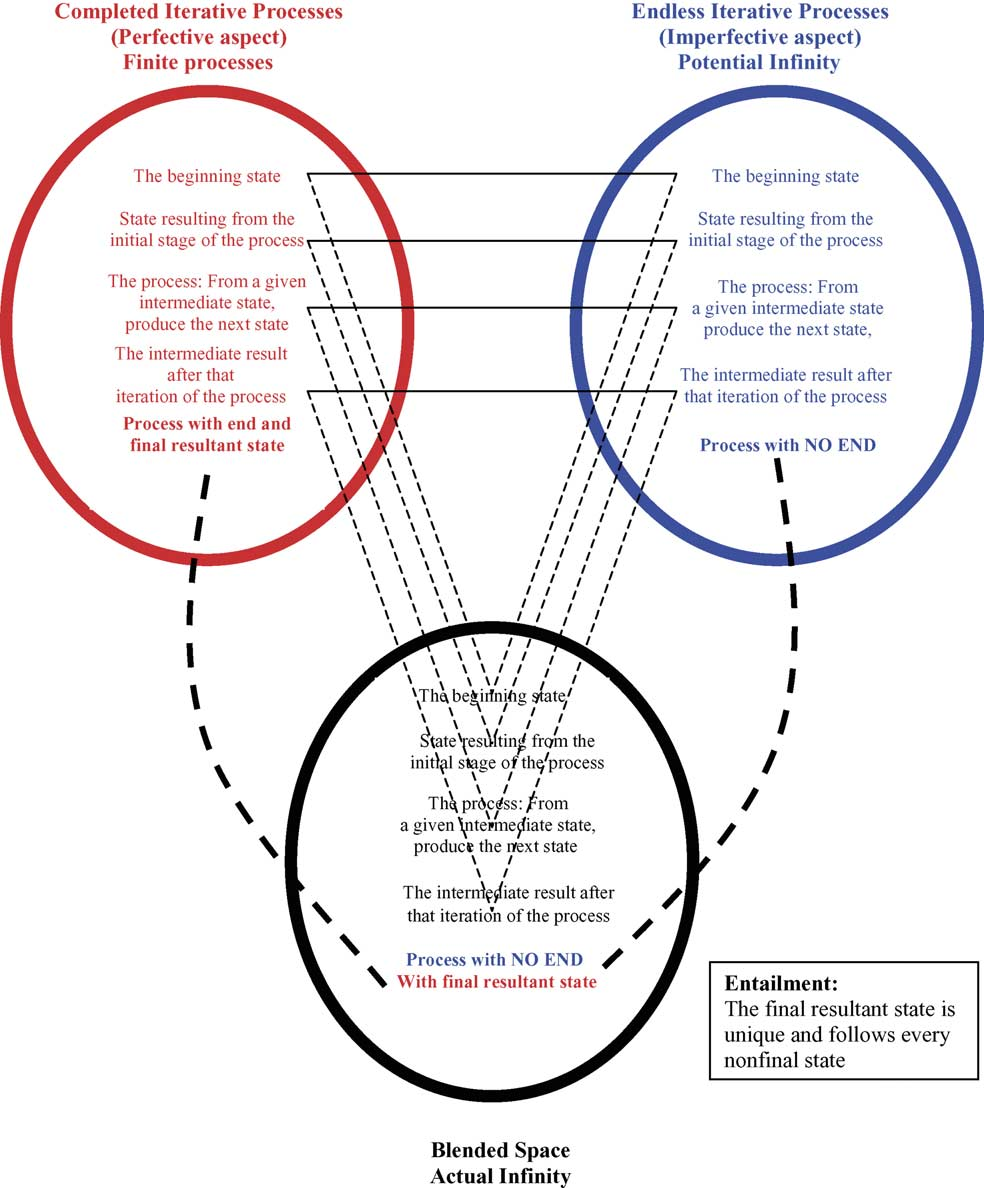
\includegraphics[width=0.4\textwidth]{transfin_nunez}  
  \caption{Blend from \textcite[p ??]{nunez05}}
  \label{fig:nunez_transfin}
\end{figure}

Figure~\ref{fig:nunez_transfin} gives an indication of the components
of the blend:
\begin{itemize}
\item The two input spaces at the top correspond to notions
of processes involving state change:
\begin{itemize}
\item  Completed Iterative Processes
are those that from some initial state, terminate in a final state
after a finite number of state transitions;
\item 
Endless Iterative Processes are those that continue indefinitely
to change state.
\end{itemize}
The marked correlations between features of the input spaces
indicate the common structure that is captured in our approach
by hte Generic Space, and as a result appear in the blend space.
\item 
Finally, the blend includes new features taken from both of the
input spaces, namely both ``process with no end'' and 
``final resultant state''.
\end{itemize}


%%% Local Variables: 
%%% mode: latex
%%% TeX-master: "mathsICCC"
%%% End: 

\section{Potential and actual infinity}

% The work of \textcite{Lak00} provides a wide range of examples of
% metaphorical reasoning in mathematics, while stressing the embodied
% cognition involved in basic mathematical experience.  

Some of the ideas of \textcite{Lak00} have been reworked by the
authors, with increased emphasis on conceptual blending.
In particular, the analysis of mathematical infinity, given in
metaphorical form as the ``Basic Metaphor of Infinity'' (BMI) in
\textcite{Lak00}, is represented in blend form in \textcite{nunez05}
as the ``Basic Mapping of Infinity'' (so, still ``BMI'').

We show here how this blend works out in our setting.
The BMI suggests that the notion of completed infinity,
in particular the possibility of transfinite numbers in the sense
of Cantor, comes from a blend of the notion of completed,
finite process with that of a potentially infinite and endless
process.

Thus take two corresponding input spaces, given by CASL specifications
\textbf{FinEnd} and \textbf{Inf} corresponding to the following diagrams


  \noindent
  \textbf{FinEnd:}
\begin{center}
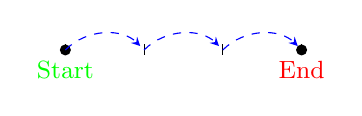
\begin{tikzpicture}[out=45,in=135,relative,>=stealth]
  \foreach \x in {0,...,3} \draw[shift={(\x,0)},color=black] (0pt,2pt)
  -- (0pt,-2pt);% node[below] {\footnotesize $\x$};
  \fill (0,0) circle (2pt); \fill (3,0) circle (2pt);

  \draw[dashed,->,color=blue,shorten >=2pt]{(0,0) to (1,0)};
  \draw[dashed,->,color=blue,shorten >=2pt]{(1,0) to (2,0)};
  \draw[dashed,->,color=blue,shorten >=2pt]{(2,0) to (3,0)};

  \node[color=red] at (3,-0.25) {\small End}; \node[color=green] at
  (0,-0.25) {\small Start};

\end{tikzpicture}
\end{center}
\noindent\textbf{Inf:} 
\begin{center}
  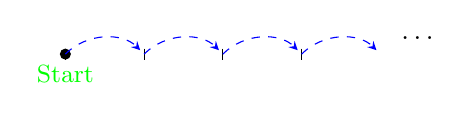
\begin{tikzpicture}[out=45,in=135,relative,>=stealth]
    \foreach \x in {0,...,3} \draw[shift={(\x,0)},color=black]
    (0pt,2pt) -- (0pt,-2pt); \fill (0,0) circle (2pt);
    % \fill (3,0) circle (2pt);

    \draw[dashed,->,color=blue,shorten >=2pt]{(0,0) to (1,0)};
    \draw[dashed,->,color=blue,shorten >=2pt]{(1,0) to (2,0)};
    \draw[dashed,->,color=blue,shorten >=2pt]{(2,0) to (3,0)};
    \draw[dashed,->,color=blue,shorten >=2pt]{(3,0) to (4,0)};

    \node at (4.5,0.2) {\dots}; \node[color=green] at (0,-0.25)
    {\small Start};

  \end{tikzpicture}
\end{center}

% \begin{figure}[h]
%   \centering
% 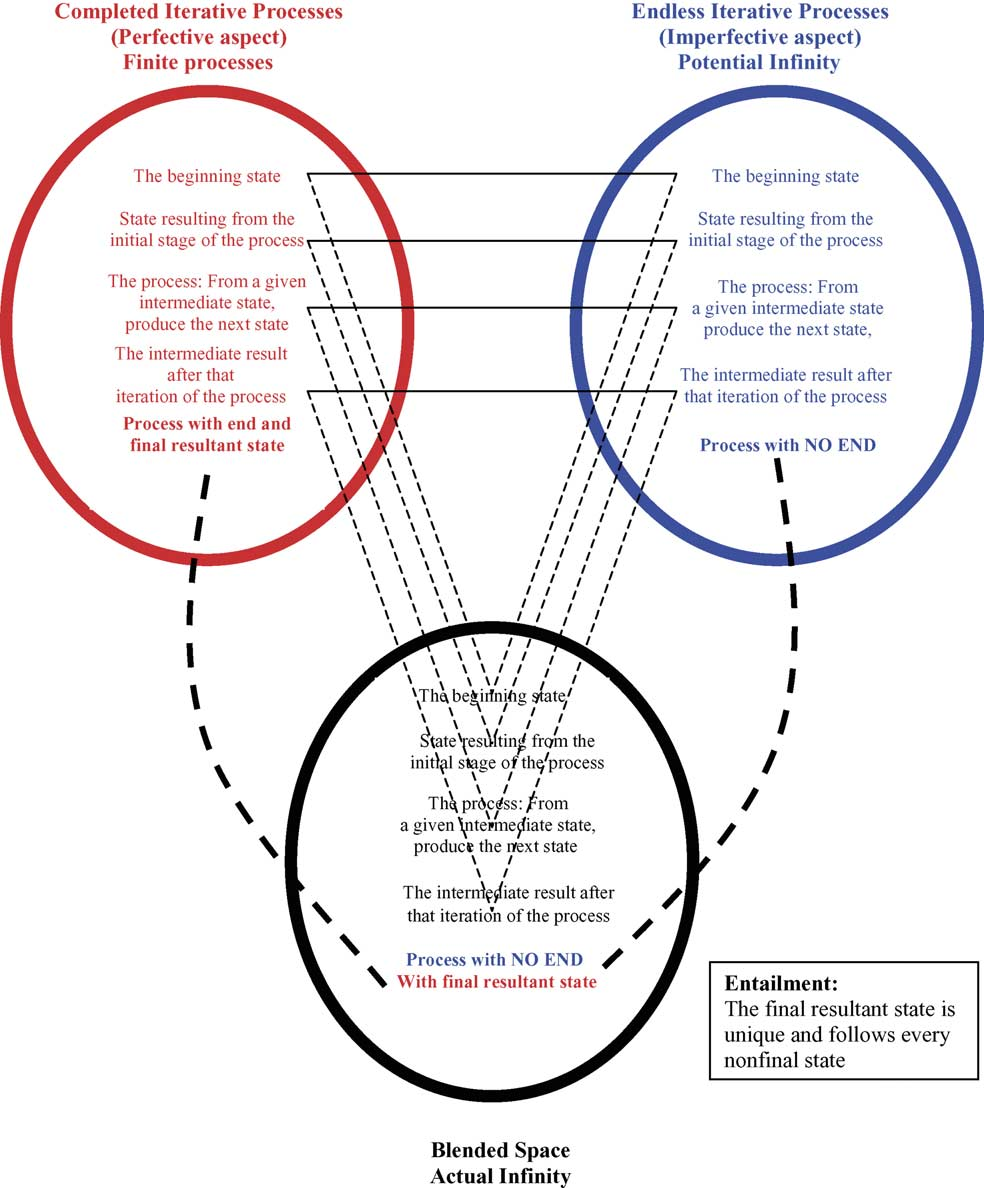
\includegraphics[width=0.4\textwidth]{transfin_nunez}  
%   \caption{Blend from \textcite[p ??]{nunez05}}
%   \label{fig:nunez_transfin}
% \end{figure}

% Figure~\ref{fig:nunez_transfin} gives an indication of the components
% of the blend:
\begin{itemize}
\item  \textbf{FinEnd:} Completed Iterative Processes
are those that from some initial state, terminate in a final state
after a finite number of state transitions.  One such case is chosen.
\item 
\textbf{Inf:} Infinite Iterative Processes are those that continue indefinitely
to change state.
\end{itemize}
In both cases, the arrows indicate steps of the processes, and
the process states are in a discrete linear order indicated by left-to-right
order in the diagrams.

The generic space \textbf{Gen} simply identifies the start states, the
notion of process step, and the linear ordering of states.

Now we can compute the blend of these spaces,
which includes new features taken from both of the
input spaces.  This blend is \emph{inconsistent}, for the
following two reasons:
\begin{enumerate}
\item the number of states is finite (from \textbf{FinEnd}), and infinite
(from \textbf{Inf});
\item  there both is an end state (from \textbf{FinEnd})
and is no end state (from \textbf{Fin}).
\end{enumerate}
Search through the possibilities of weakening the input spaces by
omitting as few axioms as possible among those involved
in an inconsistency reveals the possibility of a structure
with infinitely many states (from \textbf{Inf}) and an
end state (from \textbf{FinEnd}).  Computing the
colimit from the weakened input spaces \textbf{W-FinEnd}, \textbf{W-Inf}
gives a theory corresponding to this diagram:
\begin{center}
  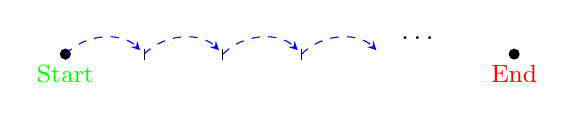
\begin{tikzpicture}[out=45,in=135,relative,>=stealth]
    \foreach \x in {0,...,3} \draw[shift={(\x,0)},color=black]
    (0pt,2pt) -- (0pt,-2pt); \fill (0,0) circle (2pt); \fill (5.7,0)
    circle (2pt);
    % \fill (3,0) circle (2pt);

    \draw[dashed,->,color=blue,shorten >=2pt]{(0,0) to (1,0)};
    \draw[dashed,->,color=blue,shorten >=2pt]{(1,0) to (2,0)};
    \draw[dashed,->,color=blue,shorten >=2pt]{(2,0) to (3,0)};
    \draw[dashed,->,color=blue,shorten >=2pt]{(3,0) to (4,0)};

    \node at (4.5,0.2) {\dots}; \node[color=green] at (0,-0.25)
    {\small Start}; \node[color=red] at (5.7,-0.25) {\small End};

  \end{tikzpicture}
\end{center}
Thus we have a blend as in the earlier examples:

%\begin{center}
%  \begin{tikzcd}[column sep=normal, row sep=small]
%    & \textrm{Colimit}
%    \\
%    \SIdIndex{W-FinEnd} \arrow{ur}{} & & \SIdIndex{W-Inf} \arrow{ul}[swap]{} \\
%    & \textrm{Gen} \arrow{ul}{}
%    \arrow{ur}[swap]{}
%  \end{tikzcd}
%\end{center}
\begin{center}
  \begin{tikzcd}[column sep=small, row sep=tiny]
    & \textrm{Colimit}
    \\
    \SIdIndex{W-FinEnd} \arrow{ur}{} & & \SIdIndex{W-Inf} \arrow{ul}[swap]{} \\
    & \textrm{Gen} \arrow{ul}{}
    \arrow{ur}[swap]{}
  \end{tikzcd}
\end{center}

   % On the other hand, if we interprete the conceptual spaces from a             
   % topological perspective \parencite{munkrestopology}, where
   % different states are in a topological space, then, the resulting       
   % blend can be clearly seen as the one-point compactification of a
   % potential infinite topological space, where the final state                
   % corresponds to the point at the infinity.


%%% Local Variables: 
%%% mode: latex
%%% TeX-master: "mathsICCC"
%%% End: 

\section{Prime Ideals as a blend}
\label{sec:prime_ideals}

\subsection*{Introduction}
One of the most fundamental concepts of modern mathematics, which is
the basis of commutative algebra and a seminal ingredient of the
language of schemes in modern algebraic geometry is the one of prime
ideal \parencite{EGAI,Eisenbud95}.

In this section, we present an implementation done in Hets
\parencite{Mossakowskihets}, in the language of CASL for the case of a
principal ideal domain (PID).  The resulting blending space contains
two equivalent definitions of the containing relation for ideals. One
of them is the trivial one in terms of elements and the other one is
given in terms of product of ideals.  It states that an ideal $X$ is
contained in an ideal $Y$ if and only if there exists an ideal $C$
such that $X=Y*C$. This is true if the base ring is a PID (it is an
elementary exercise). However, if the base ring is not a PID, for
example $R=\mathbb{Z}[T]$, then one can check that the ideals $X=(2)$
and $Y=(2,T)$ gives a counterexample.  Here, it is important to point
out that in this implementation we looked for a minimal set of axioms
such that, at the same time, the semantic interpretation can be
uniquely determined. It is always possible to construct an
implementation with additional axioms given by properties that could
be logically derived from the main axioms, (e.g. the set theoretical
properties of the containment relation for subsets of a set) but these
properties are secondary ones, meanwhile, the ones defining the
arithmetic of the ring, of an ideal and of the set of ideals of the
ring are the essential ones.

We will recover the concept of prime ideal of a
commutative ring with unity as a sort of partial (or weaken) blending
(i.e. a blend for just some axioms of the input theories) between the
concepts of an ideal of a commutative ring with unity (enriched with
the collection of all the ideals of the corresponding ring) and the
concept of a prime number of the integers.

In fact, in order to obtain the desired space it is enough to consider
a more general version of the prime numbers (in our case a partial
version), namely, a monoid $(Z,*,1)$ with an ``special'' divisibility
relation $\dannydiv$. Besides, the generic space would capture just
the syntactic correspondences that we wish to identity in the
blending space, since the blend would be basically the union of the
collection of axioms given on each space, doing the corresponding
identifications.

Our approach to blending is the one adopted by Goguen in terms of
colimits \parencite{Gog99,Goguen01,Goguen05c}.

We present the conceptual spaces from the standard ``pure'' mathematical
point of view doing concurrently the corresponding translation into
the setting of the Common Algebraic Specification Language (CASL)
\parencite{BidoitMosses2004}.

\subsection{The first conceptual space}
Let $(R,+.*,0,1)$ be a commutative ring with unity, i.e. $R$ is a set with two binary operations, $+$ and $*$, and two special elements $0,1\in R$ satisfying the following axioms:
\begin{enumerate}
\item $(\forall a\in R)(a+0=0+a=a)$
\item $(\forall a\in R)(\exists b\in R)(a+b=b+a=0)$
\item $(\forall a,b,c \in R)((a+b)+c=a+(b+c)))$
\item $(\forall a,b \in R)(a+b=b+a)$
\item $(\forall a\in R)(a*1=1*a=a)$
\item $(\forall a,b,c \in R)((a*b)*c=a*(b*c)))$
\item $(\forall a,b \in R)(a*b=b*a)$
\item $(\forall a,b,c \in R)(a*(b+c)=a*b+a*c)$
\end{enumerate}
Now, $R$ can be understood as the sort containing the elements of the corresponing commutative ring with unity.
An ideal $I$ is a subset of $R$ satisfying the following axiom:
\[(\forall i,j\in I)(\forall r\in R)(i+(-j)\in I \wedge r*i\in I).\]
\newline\indent 
Let us define a unary relation (predicate) $isideal$ on the set (sort) of subsets of $R$, $P(R)$, as follows:
$isideal(I)$ if and only if $I$ is an ideal of $R$.

Now, we define
\[{\rm Spec}_IR=\left\{A\subseteq R: isideal(A) \right\}.\]
Here, ${\rm Spec}_IR$ is considered as a subsort of the sort $P(R)$.

There is one natural operation on ${\rm Spec}_IR$, let us say
$\cdot_{\iota}$, inherited in a natural way from the corresponding
operations $+$ and $\cdot$ on $S$:

 Let $I,J\in {\rm Spec}_IR$, then we define 
%
\[I\cdot_{\iota} J:=\left\{i_1\cdot j_1+...+i_n\cdot j_n:n \in \mathbb{N} \wedge i_k\in I \wedge j_k\in J \right\}.\]

With this operation ${\rm Spec}_IR$ forms a commutative monoid
(i.e. it holds commutativity, associativity and there exists a neutral
element (in this case the ring)). However, this fact is irrelevant in
our case for the blending process. As a matter of fact, the only
property that we want to keep into the blend is the one saying that
this operation has a neutral element $1_{\iota}$, which can be seen as
an additional notation for the ring, but respect to this operation
$\cdot_{\iota}$ instead of being the sort of elements of the ring,
i.e., $R$.  \newline\indent On the other side, we want to see the
contention relation $\subseteq$ as a binary relation over the sort
${\rm Spec}_IR$.

Summarizing, our first conceptual space consists of sorts $R, {\rm Spec}_IR$ and $P(R)$; operations $+_R, *_R, 0_R, 1_R, 1_{\iota}$ and $
\cdot_{\iota}$; and the relations $\subseteq$ and $isideal$.

Here we add all the corresponding axioms defining $R$ as a commutative ring, the explicit former definition of $isideal$, ${\rm Spec}_IR$ and $\cdot_{\iota}$; and the axiom guaranteeing that  $1_{\iota}$ is the neutral element for $\cdot_{\iota}$.
 
Let us denote this space by $\mathbb{I}$.

\subsection{The second conceptual space}
Let $\mathbb{Z}$ be the set of the integer numbers. Here, we can
choose any axiomatization of them, since for the (partial) blending we
just take into account only the fact that $(\mathbb{Z},*,1)$ is a
commutative monoid. Or even simpler, we only use the fact that $1$ is
the neutral element with the operation $*$. One can, for example, take
the simple characterization of $\mathbb{Z}$, given by Martin
Brandenburg \citep{brandenburgdobleinduction}, as the only ordered
commutative ring with unity satisfying the following ``bi-inductive''
property:
\begin{align*}
  \label{eq:int}
  \forall M \subseteq \mathbb{Z}\;  & [ 0 \in M \wedge (\forall n \in \mathbb{Z} (n\in M \rightarrow n\pm 1 \in M))\\
  & \rightarrow M=\mathbb{Z}].
\end{align*}

We define also an upside down divisibility relation $\dannydiv$ defined as 
\[e\dannydiv g:=g|e,\] We re-write the classical divisibility
relation on this way in order to obtain the right primality condition
on the blend.  Let us define a unary relation $isprime$ on
$\mathbb{Z}$ as follows: for all $p\in \mathbb{Z}$, $isprime(p)$ holds
if $p\neq 1$ and the following (primality) condition holds:

\[(\forall a,b\in \mathbb{Z})(ab \dannydiv p)\rightarrow (a \dannydiv p \vee b \dannydiv p).\] 
Besides, we define the set (sort) of the prime numbers as 
\[ Prime=\left\{ p\in \mathbb{Z}/ isprime(p)\right\}\] Now, it is an
elementary fact to see that this condition is an equivalent form of
the standard definition of prime number given in the classical number
theory books (see for example \cite{Apostol76}. In the CASL language,
  we consider $\mathbb{Z}$ as the sort of the integer numbers, $*$ as
  a binary operation , $prime$ as a predicate and $\dannydiv$ as a
  binary relation, any of them defined over the sort $\mathbb{Z}$.
  \newline\indent We denote this conceptual space by $\mathbb{P}$.

\subsection{The Generic Space}

The generic space consists of a set (sort) $G$ with a binary operation $*_G$, a neutral element $S$ and a binary relation $\leq_G$.

  Let us denote this space by $\mathbb{G}$.

\subsection{The Blending Morphisms}
Now, let us define the morphisms from the generic space into the two corresponding conceptual spaces. Let $\varphi: \mathbb{G}\rightarrow \mathbb{I}$ be the morphism induced by the following syntactic correspondences $\varphi(G)={\rm Spec}_IR,\varphi(*_G)=*_{\iota}, \varphi(S)=1_{\iota}$ and $\varphi(\leq_G)=\subseteq$.
\newline\indent
Furthermore, let $\delta:=\mathbb{G}\rightarrow\mathbb{P}$ be the morphism induced by the syntactic correspondences $\delta(G)=\mathbb{Z}, \delta(*_G)=*, \delta(S)=1$ and $\delta(\leq_G)= \dannydiv$.

\subsection{The Axiomatization of the Blending}
In the every-day research of the working mathematician it happens
frequently that one starts to develop general theoretical frameworks
by combining just some aspects of two particular theories but without
considering the whole theories. For example, the development of
differential geometry was obtained combining just some aspect of
general and algebraic topology and some aspects of real analysis
\parencite{VelCad05}. The same happens with the methods use in
analytic number theory which are a fusion of some components of
elementary number theory and some of the real analysis techniques
\parencite{Apostol76}.

Therefore, it is more natural in the daily mathematical research to obtain new concepts as "partial" combinations of two former ones, i.e., as combinations (blends) of just some axioms of the corresponding two theories.
 
Thus, in our case, a partial blend will give us the desired concept. For example, from the properties defining the integers we transfer into the blend only the fact that $\mathbb{Z}$ is a set with a binary operation $*$ having $1$ as neutral element. 

So, after using the same symbols for denoting the ring as a sort of elements or as the neutral element for product of ideals $\cdot_G$, the blend has the form
\[(S, +_S, *_S, 0_S, 1_S, G={\rm Spec}_IS, isprime, Prime, \cdot_G,
S=1_G, \subseteq)\] with all the corresponding axioms of the first
conceptual space plus the translated version of the axiom defining the
primality predicate after doing the corresponding symbolic
identifications i.e., an element $P \in G$ (i.e., an ideal of $S$)
satisfied the predicate $isprime$ if and only if
\begin{align*}
P\neq S & \wedge (\forall X,Y\in G={\rm Spec}_IS). \\
        & (X\cdot_{\alpha}Y\subseteq P \rightarrow (X\subseteq P \vee Y\subseteq P)).
\end{align*}

Now, it is an elementary exercise to see that this definition is
equivalent to the fact that $P$ is a prime ideal of $S$, i.e. to the
condition
\[ P\neq S \wedge (\forall a,b\in S)(ab\in B\rightarrow (a\in P \vee
b\in P)).\] Therefore, the predicate $isprime$ turns out to be the
predicate characterizing the primality of ideals of $S$ and the set
(sort) $Prime$ turns out to be the set of prime ideals of $S$.

Besides, we just consider the fact that the up-side down divisibility
relation is a binary relation without taking into account the formal
definition into the blend.

In conclusion, the blending space consists of the axioms assuring that
$S$ is a commutative ring with unity, $G$ is the set of ideals of $S$,
$isprime$ is the predicate specifying primality for ideals of $S$ and
$Prime$ is the collection of all prime ideals of $S$.
 
\section{Implementation for the Principal Ideal Domain Case}

On this section we present an implementation done in
Hets \parencite{Mossakowskihets}, in the language of CASL for the case
of a principal ideal domain (PID).  The resulting blending space
contains two equivalent definitions of the containing relation for
ideals. One of them is the trivial one in terms of elements and the
other one is given in terms of product of ideals. It is an elementary
exercise to see this equivalence in the PID case.

%% \begin{hetcasl}
\KW{library} \Id{ideal\Ax{\_}blend}\\
\\
\KW{logic} \SId{CASL}\\
{\small{}\KW{\%\%} Prime Ideals over Principal Ideal Domains \Ax{(}PID\Ax{)} as}\\
{\small{}\KW{\%\%} Blends in Casl}\\
\\
\SPEC \=\SIdIndex{IdealsOfRing} \Ax{=}\\
\> \SORT \=\Id{RingElt}\\
\>\> {\small{}\KW{\%\%} sort of Ring Elts}\\
\> \SORT \=\Id{SubSetOfRing}\\
\>\> {\small{}\KW{\%\%} not further defined for the moment}\\
\> \PRED \=\Id{IsIdeal} \Ax{:} \Id{SubSetOfRing}\\
\>\> {\small{}\KW{\%\%} when a subset is an ideal}\\
\> \OP \=\Ax{0} \Ax{:} \Id{RingElt}\\
\> \OP \=\Ax{1} \Ax{:} \Id{RingElt}\\
\> \OP \=\Ax{\_\_}\Ax{*}\Ax{\_\_} \Ax{:} \=\Id{RingElt} \Ax{\times} \Id{RingElt} \Ax{\rightarrow} \Id{RingElt}\\
\> \OP \=\Ax{\_\_}\Ax{+}\Ax{\_\_} \Ax{:} \=\Id{RingElt} \Ax{\times} \Id{RingElt} \Ax{\rightarrow} \Id{RingElt}\\
\> \PRED \=\Ax{\_\_}\Id{isIn}\Ax{\_\_} \Ax{:} \=\Id{RingElt} \Ax{\times} \Id{SubSetOfRing}\\
\> \SORT \=\Id{Ideal} \Ax{=} \=\{\Id{I} \Ax{:} \Id{SubSetOfRing} \Ax{\bullet} \Id{IsIdeal}(\Id{I})\}\\
\> \OP \=\Id{R} \Ax{:} \Id{Ideal}\\
\>\> {\small{}\KW{\%\%} the Ring as an ideal}\\
\> \OP \=\Ax{\_\_}\Ax{**}\Ax{\_\_} \Ax{:} \=\Id{Ideal} \Ax{\times} \Id{Ideal} \Ax{\rightarrow} \Id{Ideal}, \Id{unit} \Id{R}\\
\> \PRED \=\Ax{\_\_}\Id{issubsetOf}\Ax{\_\_} \Ax{:} \=\Id{Ideal} \Ax{\times} \Id{Ideal}\\
\>\> {\small{}\KW{\%\%} partial order}\\
\>\> {\small{}\KW{\%\%}Definition of the containment predicate}\\
\> \Ax{\forall} \=\Id{A}, \Id{B} \Ax{:} \Id{Ideal} \\
\> \Ax{\bullet} \=\Id{A} \Id{issubsetOf} \Id{B} \Ax{\Leftrightarrow} \=\Ax{\forall} \Id{a} \Ax{:} \Id{RingElt} \Ax{\bullet} \=\Id{a} \Id{isIn} \Id{A} \Ax{\Rightarrow} \=\Id{a} \Id{isIn} \Id{B} \\
\> \`{\small{}\KW{\%}(subset\Ax{\_}def)\KW{\%}}\\
\> {\small{}\KW{\%\%} axioms for Ring}\\
\> \Ax{\forall} \Id{x} \Ax{:} \Id{RingElt}; \=\Id{y} \Ax{:} \Id{RingElt} \\
\> \Ax{\bullet} \=\Id{x} \Ax{+} \Id{y} \Ax{=} \=\Id{y} \Ax{+} \Id{x} \`{\small{}\KW{\%}(Commutativity\Ax{\_}\Ax{+})\KW{\%}}\\
\> \Ax{\forall} \Id{x} \Ax{:} \Id{RingElt}; \Id{y} \Ax{:} \Id{RingElt}; \=\Id{z} \Ax{:} \Id{RingElt} \\
\> \Ax{\bullet} \=(\=\Id{x} \Ax{+} \Id{y}) \Ax{+} \Id{z} \Ax{=} \=\Id{x} \Ax{+} (\=\Id{y} \Ax{+} \Id{z}) \`{\small{}\KW{\%}(Associativity \Ax{+})\KW{\%}}\\
\> \Ax{\forall} \=\Id{x} \Ax{:} \Id{RingElt} \=\Ax{\bullet} \=\Id{x} \Ax{+} \Ax{0} \Ax{=} \Id{x} \Ax{\wedge} \=\Ax{0} \Ax{+} \Id{x} \Ax{=} \Id{x} \`{\small{}\KW{\%}(unit\Ax{\_}\Ax{+})\KW{\%}}\\
\> \Ax{\forall} \=\Id{x} \Ax{:} \Id{RingElt} \=\Ax{\bullet} \=\Ax{\exists} \Id{x'} \Ax{:} \Id{RingElt} \Ax{\bullet} \=\Id{x'} \Ax{+} \Id{x} \Ax{=} \Ax{0} \`{\small{}\KW{\%}(Inverse \Ax{+})\KW{\%}}\\
\> \Ax{\forall} \Id{x} \Ax{:} \Id{RingElt}; \=\Id{y} \Ax{:} \Id{RingElt} \=\Ax{\bullet} \=\Id{x} \Ax{*} \Id{y} \Ax{=} \=\Id{y} \Ax{*} \Id{x} \`{\small{}\KW{\%}(Commutativity \Ax{*})\KW{\%}}\\
\> \Ax{\forall} \Id{x} \Ax{:} \Id{RingElt}; \Id{y} \Ax{:} \Id{RingElt}; \=\Id{z} \Ax{:} \Id{RingElt} \\
\> \Ax{\bullet} \=(\=\Id{x} \Ax{*} \Id{y}) \Ax{*} \Id{z} \Ax{=} \=\Id{x} \Ax{*} (\=\Id{y} \Ax{*} \Id{z}) \`{\small{}\KW{\%}(Associativity \Ax{*})\KW{\%}}\\
\> \Ax{\forall} \=\Id{x} \Ax{:} \Id{RingElt} \=\Ax{\bullet} \=\Id{x} \Ax{*} \Ax{1} \Ax{=} \Id{x} \Ax{\wedge} \=\Ax{1} \Ax{*} \Id{x} \Ax{=} \Id{x} \`{\small{}\KW{\%}(unit \Ax{*})\KW{\%}}\\
\> \Ax{\forall} \=\Id{x}, \Id{y}, \Id{z} \Ax{:} \Id{RingElt} \\
\> \Ax{\bullet} \=(\=\Id{x} \Ax{+} \Id{y}) \Ax{*} \Id{z} \Ax{=} \=(\=\Id{x} \Ax{*} \Id{z}) \Ax{+} (\=\Id{y} \Ax{*} \Id{z}) \`{\small{}\KW{\%}(Left\Ax{\_}Distributivity)\KW{\%}}\\
\> \Ax{\forall} \=\Id{x}, \Id{y}, \Id{z} \Ax{:} \Id{RingElt} \\
\> \Ax{\bullet} \=\Id{z} \Ax{*} (\=\Id{x} \Ax{+} \Id{y}) \Ax{=} \=(\=\Id{z} \Ax{*} \Id{x}) \Ax{+} (\=\Id{z} \Ax{*} \Id{y}) \`{\small{}\KW{\%}(Right\Ax{\_}Distributivity)\KW{\%}}\\
\> {\small{}\KW{\%\%}axioms for Ideal}\\
\> \Ax{\forall} \=\Id{I} \Ax{:} \Id{SubSetOfRing} \\
\> \Ax{\bullet} \=\Id{IsIdeal}(\Id{I}) \\
\>\> \Ax{\Leftrightarrow} \=\Ax{\forall} \Id{a}, \Id{b}, \Id{c} \Ax{:} \Id{RingElt} \\
\>\>\> \Ax{\bullet} \=(\=(\=\Id{a} \Id{isIn} \Id{I} \Ax{\Rightarrow} \=\Id{a} \Id{isIn} \Id{R}) \Ax{\wedge} \=\Ax{0} \Id{isIn} \Id{I}) \\
\>\>\>\> \Ax{\wedge} (\=\Id{a} \Id{isIn} \Id{I} \Ax{\wedge} \=\Id{c} \Id{isIn} \Id{R} \Ax{\Rightarrow} \=\Id{c} \Ax{*} \Id{a} \Id{isIn} \Id{I}) \\
\>\>\>\> \Ax{\wedge} (\=\Id{a} \Id{isIn} \Id{I} \Ax{\wedge} \=\Id{b} \Id{isIn} \Id{I} \Ax{\wedge} \=\Id{c} \Id{isIn} \Id{R} \Ax{\wedge} \=\Id{b} \Ax{+} \Id{c} \Ax{=} \Ax{0} \\
\>\>\>\>\> \Ax{\Rightarrow} \=\Id{a} \Ax{+} \Id{c} \Id{isIn} \Id{I})\\
\> \\
\> {\small{}\KW{\%\%}axioms for PID\Ax{-}s}\\
\> \PRED \=\Ax{\_\_}\Id{generates}\Ax{\_\_} \Ax{:} \=\Id{RingElt} \Ax{\times} \Id{Ideal}\\
\>\> {\small{}\KW{\%\%}an ideal is generated by an element}\\
\> \Ax{\forall} \=\Id{A} \Ax{:} \Id{Ideal} \Ax{\bullet} \=\Ax{\exists} \Id{a} \Ax{:} \Id{RingElt} \Ax{\bullet} \=\Id{a} \Id{generates} \Id{A}\\
\> \Ax{\forall} \=\Id{a} \Ax{:} \Id{RingElt} \\
\> \Ax{\bullet} \=\Ax{\forall} \Id{A} \Ax{:} \Id{Ideal} \\
\>\> \Ax{\bullet} \=\Id{a} \Id{generates} \Id{A} \\
\>\>\> \Ax{\Leftrightarrow} \=\Ax{\forall} \Id{c} \Ax{:} \Id{RingElt} \Ax{\bullet} \=\Id{c} \Id{isIn} \Id{A} \Ax{\Rightarrow} \=\Ax{\exists} \Id{d} \Ax{:} \Id{RingElt} \Ax{\bullet} \=\Id{c} \Ax{=} \=\Id{a} \Ax{*} \Id{d}\\
\> {\small{}\KW{\%\%} Definition of the product of ideals}\\
\> \Ax{\forall} \=\Id{A}, \Id{B} \Ax{:} \Id{Ideal} \\
\> \Ax{\bullet} \=\Ax{\forall} \Id{a}, \Id{b} \Ax{:} \Id{RingElt} \Ax{\bullet} \=\Id{a} \Id{isIn} \Id{A} \Ax{\wedge} \=\Id{b} \Id{isIn} \Id{B} \Ax{\Rightarrow} \=\Id{a} \Ax{*} \Id{b} \Id{isIn} \=\Id{A} \Ax{**} \Id{B}\\
\> \Ax{\bullet} \=\Ax{\forall} \Id{D} \Ax{:} \Id{Ideal} \\
\>\> \Ax{\bullet} \=(\=\Ax{\forall} \Id{a}, \Id{b} \Ax{:} \Id{RingElt} \Ax{\bullet} \=\Id{a} \Id{isIn} \Id{A} \Ax{\wedge} \=\Id{b} \Id{isIn} \Id{B} \Ax{\Rightarrow} \=\Id{a} \Ax{*} \Id{b} \Id{isIn} \=\Id{A} \Ax{**} \Id{B}) \\
\>\>\> \Ax{\Rightarrow} \=\Id{A} \Ax{**} \Id{B} \Id{issubsetOf} \Id{D}\\
\KW{end}\\
{\small{}\KW{\%\%} axioms defining a very simple version of the integers\Ax{,}}\\
{\small{}\KW{\%\%} considered with an operation \Ax{*}\Ax{,} a binary relation \Ax{|}\Ax{|}}\\
{\small{}\KW{\%\%} \Ax{(}upside\Ax{-}down divisibility relation\Ax{)} and a primality axiom\Ax{.}}\\
\\
\SPEC \=\SIdIndex{SimpleInt} \Ax{=}\\
\> \SORT \Id{SimpleElem}\\
\> \OPS \=\Ax{1} \Ax{:} \Id{SimpleElem};\\
\>\> \Ax{\_\_}\Id{x}\Ax{\_\_} \Ax{:} \=\Id{SimpleElem} \Ax{\times} \Id{SimpleElem} \Ax{\rightarrow} \Id{SimpleElem}, \\
\>\> \Id{comm}, \Id{assoc}, \Id{unit} \Ax{1}\\
\> \PREDS \=\Ax{\_\_}\Ax{||}\Ax{\_\_} \Ax{:} \=\Id{SimpleElem} \Ax{\times} \Id{SimpleElem};\\
\>\> {\small{}\KW{\%\%} division gives partial order}\\
\>\> \Id{IsPrime} \Ax{:} \Id{SimpleElem}\\
\> \Ax{\forall} \=\Id{x}, \Id{y} \Ax{:} \Id{SimpleElem} \\
\> \Ax{\bullet} \=\Id{x} \Ax{||} \Id{y} \Ax{\Leftrightarrow} \=\Ax{\exists} \Id{c} \Ax{:} \Id{SimpleElem} \Ax{\bullet} \=\Id{x} \Ax{=} \=\Id{y} \Id{x} \Id{c}\\
\> {\small{}\KW{\%}\KW{Def\_upsidedownDivisilityRelation}\Ax{\%}}\\
\> {\small{}\KW{\%\%} subsort of primes}\\
\> \SORT \=\Id{SimplePrime} \Ax{=} \=\{\Id{p} \Ax{:} \Id{SimpleElem} \Ax{\bullet} \Id{IsPrime}(\Id{p})\}\\
\> \Ax{\forall} \=\Id{p} \Ax{:} \Id{SimpleElem} \\
\> \Ax{\bullet} \=\Id{IsPrime}(\Id{p}) \\
\>\> \Ax{\Leftrightarrow} \=(\=\Ax{\forall} \Id{a}, \Id{b} \Ax{:} \Id{SimpleElem} \Ax{\bullet} \=\Id{a} \Id{x} \Id{b} \Ax{||} \Id{p} \Ax{\Rightarrow} \=\Id{a} \Ax{||} \Id{p} \Ax{\vee} \=\Id{b} \Ax{||} \Id{p}) \Ax{\wedge} \Ax{\neg} \=\Id{p} \Ax{=} \Ax{1}\\
\> {\small{}\KW{\%}\KW{Def\_primality}\Ax{\%}}\\
\KW{end}\\
{\small{}\KW{\%\%} Generic space}\\
\\
\SPEC \=\SIdIndex{Gen} \Ax{=}\\
\> \SORT \Id{Generic}\\
\> \OPS \=\Id{S} \Ax{:} \Id{Generic};\\
\>\> \Ax{\_\_}\Id{gpr}\Ax{\_\_} \Ax{:} \=\Id{Generic} \Ax{\times} \Id{Generic} \Ax{\rightarrow} \Id{Generic}, \Id{unit} \Id{S}\\
\> \PRED \=\Id{gcont} \Ax{:} \=\Id{Generic} \Ax{\times} \Id{Generic}\\
\KW{end}\\
\\
\VIEW \=\SId{I1} \Ax{:} \\
\> \SId{Gen} \KW{to} \SId{IdealsOfRing} \Ax{=} \\
\> \Id{Generic} \Ax{\mapsto} \Id{Ideal}, \Id{S} \Ax{\mapsto} \Id{R}, \Ax{\_\_}\Id{gpr}\Ax{\_\_} \Ax{\mapsto} \=\Ax{\_\_}\Ax{**}\Ax{\_\_}, \\
\> \Id{gcont} \Ax{\mapsto} \=\Ax{\_\_}\Id{issubsetOf}\Ax{\_\_}\\
\KW{end}\\
\\
\VIEW \=\SId{I2} \Ax{:} \\
\> \SId{Gen} \KW{to} \SId{SimpleInt} \Ax{=} \\
\> \Id{Generic} \Ax{\mapsto} \Id{SimpleElem}, \Id{S} \Ax{\mapsto} \Ax{1}, \Ax{\_\_}\Id{gpr}\Ax{\_\_} \Ax{\mapsto} \=\Ax{\_\_}\Id{x}\Ax{\_\_}, \\
\> \Id{gcont} \Ax{\mapsto} \=\Ax{\_\_}\Ax{||}\Ax{\_\_}\\
\KW{end}\\
\\
\SPEC \=\SIdIndex{Colimit} \Ax{=}\\
\> \KW{combine} \=\Id{I1}, \Id{I2}\\
\KW{end}
\end{hetcasl}


After computing the corresponding colimit in HETS and after
interpreting ``RingEl'' as the sort containing the elements of the ring
$S$, the theory defining the blend corresponds to the axioms defining
a PID (S), the set of all its ideals (Generic) and the set all its
prime ideals (SimplePrime):

%% \begin{hetcasl}
% \KW{library} \Id{ideal\Ax{\_}colim}\\
% \\
% \KW{logic} \SId{CASL}\Id{\Ax{.}}\SId{SulFOL=}\\
% \\
\SPEC \=\SIdIndex{Spec} \Ax{=}\\
\> \SORTS \=\Id{Generic}, \Id{RingElt}, \Id{SimplePrime}, \Id{SubSetOfRing}\\
\> \SORTS \=\Id{SimplePrime} \Ax{<} \Id{Generic};\\
\>\> \Id{Generic} \Ax{<} \Id{SubSetOfRing}\\
\> \OP \=\Ax{0} \Ax{:} \Id{RingElt}\\
\> \OP \=\Ax{1} \Ax{:} \Id{RingElt}\\
\> \OP \=\Id{S} \Ax{:} \Id{Generic}\\
\> \OP \=\Ax{\_\_}\Ax{*}\Ax{\_\_} \Ax{:} \=\Id{RingElt} \Ax{\times} \Id{RingElt} \Ax{\rightarrow} \Id{RingElt}\\
\> \OP \=\Ax{\_\_}\Ax{+}\Ax{\_\_} \Ax{:} \=\Id{RingElt} \Ax{\times} \Id{RingElt} \Ax{\rightarrow} \Id{RingElt}\\
\> \OP \=\Ax{\_\_}\Id{x}\Ax{\_\_} \Ax{:} \=\Id{Generic} \Ax{\times} \Id{Generic} \Ax{\rightarrow} \Id{Generic}\\
\> \PRED \=\Id{IsIdeal} \Ax{:} \Id{SubSetOfRing}\\
\> \PRED \=\Id{IsPrime} \Ax{:} \Id{Generic}\\
\> \PRED \=\Ax{\_\_}\Id{isIn}\Ax{\_\_} \Ax{:} \=\Id{RingElt} \Ax{\times} \Id{SubSetOfRing}\\
\> \PRED \=\Id{gcont} \Ax{:} \=\Id{Generic} \Ax{\times} \Id{Generic}\\
\> \PRED \=\Ax{\_\_}\Id{generates}\Ax{\_\_} \Ax{:} \=\Id{RingElt} \Ax{\times} \Id{Generic}\\
\> \Ax{\forall} \=\Id{I} \Ax{:} \Id{SubSetOfRing} \Ax{\bullet} \=\Id{I} \Ax{\in} \Id{Generic} \Ax{\Leftrightarrow} \Id{IsIdeal}(\Id{I})\\
\> \Ax{\forall} \=\Id{x} \Ax{:} \Id{Generic} \Ax{\bullet} \=\Id{x} \Id{x} \Id{S} \Ax{=} \Id{x}\\
\> \Ax{\forall} \=\Id{x} \Ax{:} \Id{Generic} \Ax{\bullet} \=\Id{S} \Id{x} \Id{x} \Ax{=} \Id{x}\\
\> \Ax{\forall} \=\Id{A}, \Id{B} \Ax{:} \Id{Generic} \\
\> \Ax{\bullet} \=\Id{gcont}(\=\Id{A}, \Id{B}) \Ax{\Leftrightarrow} \=\Ax{\forall} \Id{a} \Ax{:} \Id{RingElt} \Ax{\bullet} \=\Id{a} \Id{isIn} \Id{A} \Ax{\Rightarrow} \=\Id{a} \Id{isIn} \Id{B}\\
\> \Ax{\forall} \=\Id{x}, \Id{y} \Ax{:} \Id{RingElt} \Ax{\bullet} \=\Id{x} \Ax{+} \Id{y} \Ax{=} \=\Id{y} \Ax{+} \Id{x}\\
\> \Ax{\forall} \=\Id{x}, \Id{y}, \Id{z} \Ax{:} \Id{RingElt} \Ax{\bullet} \=(\=\Id{x} \Ax{+} \Id{y}) \Ax{+} \Id{z} \Ax{=} \=\Id{x} \Ax{+} (\=\Id{y} \Ax{+} \Id{z})\\
\> \Ax{\forall} \=\Id{x} \Ax{:} \Id{RingElt} \Ax{\bullet} \=\Id{x} \Ax{+} \Ax{0} \Ax{=} \Id{x} \Ax{\wedge} \=\Ax{0} \Ax{+} \Id{x} \Ax{=} \Id{x}\\
\> \Ax{\forall} \=\Id{x} \Ax{:} \Id{RingElt} \Ax{\bullet} \=\Ax{\exists} \Id{x'} \Ax{:} \Id{RingElt} \Ax{\bullet} \=\Id{x'} \Ax{+} \Id{x} \Ax{=} \Ax{0}\\
\> \Ax{\forall} \=\Id{x}, \Id{y} \Ax{:} \Id{RingElt} \Ax{\bullet} \=\Id{x} \Ax{*} \Id{y} \Ax{=} \=\Id{y} \Ax{*} \Id{x}\\
\> \Ax{\forall} \=\Id{x}, \Id{y}, \Id{z} \Ax{:} \Id{RingElt} \Ax{\bullet} \=(\=\Id{x} \Ax{*} \Id{y}) \Ax{*} \Id{z} \Ax{=} \=\Id{x} \Ax{*} (\=\Id{y} \Ax{*} \Id{z})\\
\> \Ax{\forall} \=\Id{x} \Ax{:} \Id{RingElt} \Ax{\bullet} \=\Id{x} \Ax{*} \Ax{1} \Ax{=} \Id{x} \Ax{\wedge} \=\Ax{1} \Ax{*} \Id{x} \Ax{=} \Id{x}\\
\> \Ax{\forall} \=\Id{x}, \Id{y}, \Id{z} \Ax{:} \Id{RingElt} \Ax{\bullet} \=(\=\Id{x} \Ax{+} \Id{y}) \Ax{*} \Id{z} \Ax{=} \=(\=\Id{x} \Ax{*} \Id{z}) \Ax{+} (\=\Id{y} \Ax{*} \Id{z})\\
\> \Ax{\forall} \=\Id{x}, \Id{y}, \Id{z} \Ax{:} \Id{RingElt} \Ax{\bullet} \=\Id{z} \Ax{*} (\=\Id{x} \Ax{+} \Id{y}) \Ax{=} \=(\=\Id{z} \Ax{*} \Id{x}) \Ax{+} (\=\Id{z} \Ax{*} \Id{y})\\
\> \Ax{\forall} \=\Id{I} \Ax{:} \Id{SubSetOfRing} \\
\> \Ax{\bullet} \=\Id{IsIdeal}(\Id{I}) \\
\>\> \Ax{\Leftrightarrow} \=\Ax{\forall} \Id{a}, \Id{b}, \Id{c} \Ax{:} \Id{RingElt} \\
\>\>\> \Ax{\bullet} \=(\=(\=\Id{a} \Id{isIn} \Id{I} \Ax{\Rightarrow} \=\Id{a} \Id{isIn} \Id{S}) \Ax{\wedge} \=\Ax{0} \Id{isIn} \Id{I}) \\
\>\>\>\> \Ax{\wedge} (\=\Id{a} \Id{isIn} \Id{I} \Ax{\wedge} \=\Id{c} \Id{isIn} \Id{S} \Ax{\Rightarrow} \=\Id{c} \Ax{*} \Id{a} \Id{isIn} \Id{I}) \\
\>\>\>\> \Ax{\wedge} (\=\Id{a} \Id{isIn} \Id{I} \Ax{\wedge} \=\Id{b} \Id{isIn} \Id{I} \Ax{\wedge} \=\Id{c} \Id{isIn} \Id{S} \Ax{\wedge} \=\Id{b} \Ax{+} \Id{c} \Ax{=} \Ax{0} \\
\>\>\>\>\> \Ax{\Rightarrow} \=\Id{a} \Ax{+} \Id{c} \Id{isIn} \Id{I})\\
\> \Ax{\forall} \Id{a} \Ax{:} \Id{RingElt}; \=\Id{A} \Ax{:} \Id{Generic} \\
\> \Ax{\bullet} \=\Id{a} \Id{generates} \Id{A} \\
\>\> \Ax{\Leftrightarrow} \=\Ax{\forall} \Id{c} \Ax{:} \Id{RingElt} \Ax{\bullet} \=\Id{c} \Id{isIn} \Id{A} \Ax{\Rightarrow} \=\Ax{\exists} \Id{d} \Ax{:} \Id{RingElt} \Ax{\bullet} \=\Id{c} \Ax{=} \=\Id{a} \Ax{*} \Id{d}\\
\> \Ax{\forall} \Id{A}, \Id{B} \Ax{:} \Id{Generic}; \=\Id{a}, \Id{b} \Ax{:} \Id{RingElt} \\
\> \Ax{\bullet} \=\Id{a} \Id{isIn} \Id{A} \Ax{\wedge} \=\Id{b} \Id{isIn} \Id{B} \Ax{\Rightarrow} \=\Id{a} \Ax{*} \Id{b} \Id{isIn} \=\Id{A} \Id{x} \Id{B}\\
\> \Ax{\forall} \=\Id{A}, \Id{B}, \Id{D} \Ax{:} \Id{Generic} \\
\> \Ax{\bullet} \=(\=\Ax{\forall} \Id{a}, \Id{b} \Ax{:} \Id{RingElt} \Ax{\bullet} \=\Id{a} \Id{isIn} \Id{A} \Ax{\wedge} \=\Id{b} \Id{isIn} \Id{B} \Ax{\Rightarrow} \=\Id{a} \Ax{*} \Id{b} \Id{isIn} \Id{D}) \\
\>\> \Ax{\Rightarrow} \Id{gcont}(\=\Id{A} \Id{x} \Id{B}, \Id{D})\\
\> \Ax{\forall} \=\Id{x}, \Id{y} \Ax{:} \Id{Generic} \Ax{\bullet} \=\Id{gcont}(\=\Id{x}, \Id{y}) \Ax{\Leftrightarrow} \=\Ax{\exists} \Id{c} \Ax{:} \Id{Generic} \Ax{\bullet} \=\Id{x} \Ax{=} \=\Id{y} \Id{x} \Id{c}\\
\> \Ax{\forall} \=\Id{p} \Ax{:} \Id{Generic} \Ax{\bullet} \=\Id{p} \Ax{\in} \Id{SimplePrime} \Ax{\Leftrightarrow} \Id{IsPrime}(\Id{p})\\
\> \Ax{\forall} \=\Id{p} \Ax{:} \Id{Generic} \\
\> \Ax{\bullet} \=\Id{IsPrime}(\Id{p}) \\
\>\> \Ax{\Leftrightarrow} \=(\=\Ax{\forall} \Id{a}, \Id{b} \Ax{:} \Id{Generic} \\
\>\>\>\> \Ax{\bullet} \=\Id{gcont}(\=\Id{a} \Id{x} \Id{b}, \Id{p}) \Ax{\Rightarrow} \=\Id{gcont}(\=\Id{a}, \Id{p}) \Ax{\vee} \Id{gcont}(\=\Id{b}, \Id{p})) \\
\>\>\> \Ax{\wedge} \Ax{\neg} \=\Id{p} \Ax{=} \Id{S}\\
\KW{end}
\end{hetcasl}


The details of this implementation can be consulted at \texttt{somewhere/on/line}.


%%% Local Variables: 
%%% mode: latex
%%% TeX-master: "mathsICCC"
%%% End: 


\section{A Challenge Example for Blending} \label{galois}

\subsection{Computational Creativity via Blending}

The examples shown thus far in the paper have been examples of
blending in mathematics whose mechanisation has helped to identify
some novel and unexpected results. The blending itself was a one-stage
process where human input was required to identify the input
concepts. A more ambitious aim of the approach of applying blending to
the problem of computational creativity in mathematics, is to allow
search to be done over multiple blends and for the {\em process} of
blending to be controlled mechanically. In this section we describe
very informally a mathematical domain to which a process of blends may
be appicable.

\subsection{Galois Theory}
% Danny, Joe, Felix, Ewen

This example is developed in a less formal manner than the previous.
It is included both to highlight some outstanding technical issues,
and to develop some broader theoretical points about the future
prospects and applications of our approach.  

In its most straightforward formulation, Galois theory develops a
relationship between a polynomial $f(x)$ with coefficients in some
field $F$, the extension of $K$ of $F$ (written ``$K/F$'') containing
all of the roots of $f(x)$, and the group $\mathbf{Gal}(K)$ of
automorphisms of $K/F$ that fix the elements of $F$.  The fundamental
theorem of Galois theory states that there is a bijection between the
subfields of $K/F$ and the subgroups of $\mathbf{Gal}(K)$;
namely, subgroups correspond to their fixed fields.  Using this
correspondence, properties of polynomials can be derived, most
famously the fact that quintic polynomials cannot be solved by
algebraic operations and the extraction of roots.  

We do not propose to reconstruct much of the theory here, but note
that already in this basic account there are several steps that seem
compellingly ``blend-like.''

In the first place, that would describes the notion of a field
extension quite well.  $E$ is an extension of $F$ if $E \supseteq F$.
We could derive the extension relationship from the input concepts $E$
and $F$ by ``taking everything additional from $E$ and adding it to
$F$.''  This is made specific in the process of \emph{adjoining}
elements to a field, which simply means to augment the field with all
formal finite sums and products of the adjoined elements with
coefficients in the base field.

Second, the notion of the \emph{splitting field} of a polynomial,
namely the special extension $K/F$ containing all of the roots of
$f(x)$.  This could be formed conceptually by combining the concept
``\emph{the roots of a polynomial $f$ with coefficients in a field
  $F$}'' and the concept ``\emph{a field extension $E/F$ formed by
  adjoining certain elements to $F$}.''  Formally, the roots of $f$
are not part of in the second concept, and they must be put in
correspondence with the ``certain elements.''  Note that formulating
the concept of a splitting field in this way is different from proving
that a splitting field always exists.  It does, however, and the proof
(by induction on the degree of the polynomial) works by successively
adjoining elements to $F$.  This gives an inkling of the idea that
blending could be used as a proof step.

As above, we could then form the concept of $\mathbf{Gal}(K)$ by blending
at the conceptual level.  This time, there would be several constituent pieces:
``\emph{the roots of a polynomial $f$ with coefficients in a field $F$},''
``\emph{the splitting field of $f$},''
``\emph{the group of automorphisms of a field extension $E$},''
``\emph{the automorphisms that fix $F$}.''

Finally, assuming that we have built $\mathbf{Gal}(K)$ in this
fashion, we would like to know some of its properties.  Consider the
claim that \emph{elements of $\mathbf{Gal}(K)$ permute the roots of
  $f$}.  This time, instead of being purely conceptual, we want to
work at the \emph{process} level, and consider before-and-after
descriptions of the result of applying $\varphi\in\mathbf{Gal}(K)$ to
some $r$ with the property $f(r)=0$.  This is similar in some ways to
the ``Riddle of the Buddhist Monk'' \cite{Fau98} which is cited as
an example of the power of blending.\footnote{Fauconnier and Turner
  cite Arthur Koestler: ``A Buddhist monk begins at dawn one day
  walking up a mountain, reaches the top at sunset, meditates at the
  top for several days until one dawn when he begins to walk back to
  the foot of the mountain, which he reaches at sunset.  Making no
  assumptions about his starting or stopping or about his pace during
  the trips, prove that there is a place on the path which he occupies
  at the same hour of the day on the two separate journeys.''}
However, this time the generic space is not a simple geometric machine,
but rather an algebraic machine with several moving parts.

The proof of the claim is as follows.  If $f(r)=0$, then $\varphi
f(r)=\varphi 0$.  Since $\varphi$ is an automorphism, $\varphi 0 = 0$;
and furthermore $\varphi$ distributes over the sums and products that
make up the polynomial $f$ and fixes its coefficients, therefore
$\varphi f(r)=f(\varphi r)$.  Chaining the equalities together, we
have $f(\varphi r)=0$.

In short, the proof is a fairly direct result of combining ``what it
means to be a root,'' ``what it means to be an automorphism,''
``what it means to say that the automorphism fixes elements of $F$,''
and
``what it means to be a polynomial with coefficients in the
field $F$.''
Indeed, the proof is in some sense the only thing it could be if one
knows the definitions.  

\textcite{Goguen92sheafsemantics} suggests that ``combination is
colimit.''  Can we realise the proof through (one or several) colimit
operations?  I.e.~is the proof a blend?  And is there anything special
about this proof?

\subsection{Issues raised}

We have investigated the possibility of formalising Galois theory, and
note here some of the possibilties for blend computations, along with
some issues we need to address.

\subsubsection{Field Extension as a Blend}

The first possibility here is that one could exploit blending
machinery in order to discover the notion of a field extension. Take a
field $F$ and adjoining it with an element $a$ to form $F(a)$ is a
form of a blend of the conceptual space containing the field $F$ and
the conceptual space containing element $a$. Equally for a field
extension one could envisage blending a conceptual space containing
field $F$ with a conceptual space containing a set of elements
$E$. The field axioms then hold for $F$ and $E/F$, but not for the
elements of $E$.

Although this seems a natural blend, in reality when reasoning about
polynomials with rational coefficients, it is useful to distinguish
the three separate types -- those of $E$, those of $F$ and those of
$E/F$ as a supertype. Using blending machinery removes the distinction
between these types.

\subsubsection{Splitting Field Extension Theorem}

We would like to be able to use blending to discover that there exists a
field $F$ extended with roots of polynomial $f(x)$, where the coefficients of $f(x)$ are in $F$. The more challenging but creative step is to discover that extending $F$ {\em only} with the roots of $f(x)$ forms a field. We have investigated the possibility of blending the concept of the root of a polynomial with rational coefficients with a field of rationals and then trying to prove these theorem from the resulting axioms. Discovery of the thoerem itself is the real creative step and is an example of running the blend. This is ambitious and is further work.

\subsubsection{Automorphisms}

In order to discover the most interesting and surprising Galois
theorem, that automorphisms fixing the field $F$ permute the elements
of $E$ in field extension $E/F$, we need to be able formalise the
notion of an automorphism. The most natural way to do this is in the
machinery that we currently use is to define an automorphism $\alpha$
as a higher order function: $\alpha:\; E/F \to E/F$. Currently there
is no way of computing colimits with higher order symbols
mechanically, so we are constrained to do this on paper.
%% There are various technical questions \textbf{(@Alan, @Ewen, @Felix)},
%% but from a naive mathematical standpoint the first issue is: is it
%% always clear how to combine the relevant facts?  And a related
%% question: is it always clear what the relevant facts actually are?

%% If blending is the realisation of ``combinatorial creativity'' why are
%% we not swamped by the combinatorial explosion of possible things to
%% combine?

%% \textbf{[JC: 1/4 page to flesh out the details.]}
%%  \newpage

%%% Local Variables: 
%%% mode: latex
%%% TeX-master: "mathsICCC"
%%% End: 

\section{Evaluation and Outlook}
\label{sec:eval}

\subsection{Review of the current offering}

\begin{itemize}
\item[(a)] We began the paper with the reconstruction of certain
mathematical objects, showing the technical feasibility of the
approach. 
\item[(b)] The more advanced example at the centre of the paper
  illustrates how this sort of reconstruction relates to mathematical
  practice.
\item[(c)] A future-oriented example exposes some technical
  challenges, while suggesting that blending could offer a novel
  approach to computer mathematics.
\end{itemize}

\subsection{Broader issues in evaluation}

In addition to motivating a further investigation of the role blending
can play in proofs, Galois theory, discussed above, is paradigmatic
for other reasons.  This discussion draws on the early 20th Century
writings of Albert Lautman on the philosophy of mathematics and the
subsequent interpretation of this work by Gilles Deleuze.  It uses
these ideas to propose an approach to embedding evaluation within the
system itself.

Concerning the common features of Galois theory, class field theory,
and the development of the universal covering surface in Riemann
geometry, \cite[p. 126]{lautman2011mathematics} writes:
\begin{quote}
What is characteristic of the movement of the theories that will be
considered here is the existence of an end conceived in advance as a
term of the ascent.
\end{quote}

% This is reminiscent of our notion of coherence criteria that apply to
This is reminiscent of our notion of internal evaluation that apply to
the blend.  To illustrate, let us briefly imagine how we would use
blending techniques to move from porcupine+lion to the perfected
\emph{porculione}.  Here, instead of field automorphisms that preserve
mathematical structure and fix certain designated elements, we would
look for mappings that preserve other properties that exist in the
underlying domain.  Porculiones would presumably have four feet, would
be mammals, and would be omnivores; they should also be viable living
creatures.

\cite[pp. 227--228]{deleuze1994difference} follows
Lautman in enthusiastically endorsing the Galoisian approach to
mathematics:
\begin{quote}
[T]he fact that an equation cannot be solved algebraically, for
example, is no longer discovered as a result of empirical research or
by trial and error, but as a result of the characteristics of the
groups and partial resolvents which constitute the synthesis of the
problem and its conditions (an equation is solveable only by algebraic
means -- in other words, by radicals, when the partial resolvents are
binomial equations and the indices of the groups are prime numbers).
The theory of problems is completely transformed and at last grounded,
since we are no longer in the classic master-pupil situation where the
pupil understands and follows a problem only to the extent that the
master already knows the solution and provides the necessary
adjunctions.  For, as Georges Verriest remarks, the group of an
equation does not characterise at a given moment what we know about
its roots, but the objectivity of what we do not know about them.
Conversely, this non-knowledge is no longer a negative or an
insufficiency but a rule or \emph{something to be learnt} which
corresponds to a fundamental dimension of the object.
\end{quote}

Although there is a commonality between blending and the
Galoisian approach insofar as progressive refinement carries us toward a
``perfected'' conclusion, Deleuze's enthusiasm about the pedagogical
situation would be significantly cooled here.  It would seem, in many
of our examples, that we only make progress ``to the extent that the
master already knows the solution and provides the necessary
adjunctions.''

However, this apparent infelicity may be less of a thick obstacle than
it would initially appear.  What seems to be most needed is a notion
of a \emph{question} inside the system.  This would recover Lautman's
basic thrust: ``Scientific or not, every question has built in some
assumptions about the form of the answer'' \cite{larvor2011albert}.
In short, an experimental approach in which the system \emph{asks} and
\emph{answers} questions would embed key aspects evaluation in the
system itself.

\subsection{Future work}

The idea of using blending to carry out steps in a proof would provide
a useful training ground for further development.  The primary problem
is: If blending is the realisation of ``combinatorial creativity'' how
will we avoid being swamped by the combinatorial explosion of possible
things to combine?  The first challenge is thus fitting different
mathematical components together in a sensible manner.  A related
challenge would apply when modifying the system to selectively
experiment with the rules it uses.  The objective in this case would
be for the system to learn to associate different (useful) techniques
with different types of problems.
%% Some reference to the music and other technology for blending here?

%%% Local Variables: 
%%% mode: latex
%%% TeX-master: "mathsICCC"
%%% End: 

\section{Conclusions and Remarks}
\label{sec:conc}

The examples presented in this paper trace the development of the
blending approach.
The current paper begins with reconstructions, but also
quickly shows how computed blends can suggest new mathematical
definitions and concepts of interest to practising mathematicians.
The analysis offered here shows that this work is a building block that
will be useful for future developments that are able to reason more
flexibly about mathematical problems -- and systematically find and
propose new concepts and problems.

In future work, we will look more at the cognitive issues raised in
this work. In particular, the use of \emph{image schemas} can give a
link between the computational and representational approach taken
here, and the cognitive claims coming from authors such as Fauconnier
and Turner, and Johnson.  Here the work of \textcite{ManPag14} and
\textcite{HeKuNe14short} gives an idea of how these underlying
cognitive primitives can be expressed in logical form, and can thus
play an explicit role in our modelling of creativity in mathematics.


%%% Local Variables: 
%%% mode: latex
%%% TeX-master: "mathsICCC"
%%% End: 


\nocite{Weil60}
% \nocite{Boden90}
\nocite{nunez05}
\nocite{Lak00}
\nocite{Gog05,Gog99}

\printbibliography

\end{document}
